%%%%%%%%%%%%%%%%%%%%%%%%%%%%%%%%%%%%%%%%%%%
%%%%%%%%%%%%%%%%%%%%%%%%%%%%%%%%%%%%%%%%%%%
%%%%%%%%%%%%%%%%%%%%%%%%%%%%%%%%%%%%%%%%%%%


%%%%%%%%%%%%%%%%%%%%%%%%%%%%%%%%%%%%%%%%%%%
%%%%%%%%%%%%%%%%%%%%%%%%%%%%%%%%%%%%%%%%%%%
%%%%%%%%%%%%%%%%%%%%%%%%%%%%%%%%%%%%%%%%%%%
%%%%%%%%%%%%%%%%%%%%%%%%%%%%%%%%%%%%%%%%%%%
%%%%%%%%%%%%%%%%%%%%%%%%%%%%%%%%%%%%%%%%%%%
%%%%%%%%%%%%%%%%%%%%%%%%%%%%%%%%%%%%%%%%%%%

\chapter{beautiful graphics ggplot2}
\textcolor{white}{.}\newline
\textbf{Auteur : } C.J. Liu\newline
\textbf{Date : } 11/17/2016\newline
\textbf{Lien: } \underline{\href{https://rstudio-pubs-static.s3.amazonaws.com/228019\_f0c39e05758a4a51b435b19dbd321c23.html\#11\_area\_plots}{ici}}\newline

\section{Plot One Variable - X : Continuous or Discrete}
For \textbf{one continuous variable = Numeric} :
\begin{itemize}
  \item geom\_area()
  \item geom\_density()
  \item geom\_histogram()
  \item geom\_freqpoly()
  \item geom\_dotplot()
  \item stat\_ecdf()
  \item stat\_qq()
\end{itemize}
For \textbf{one discrete varaible = Factor} :

\begin{itemize}
  \item geom\_bar()
\end{itemize}

\begin{lstlisting}[language=html]
> library(ggplot2)
> library(dplyr)
\end{lstlisting}
\subsection{Area Plots}
\textbf{alpha, color, fill, linetype, size}
\begin{lstlisting}[language=html]
> set.seed(1234)
> wdata = as_data_frame(data.frame(sex = factor(rep(c("F", "M"), each=200)), weight = c(rnorm(200,55),rnorm(200,58))))
> wdata
# A tibble: 400 x 2
      sex   weight
   <fctr>    <dbl>
 1      F 53.79293
 2      F 55.27743
 3      F 56.08444
 4      F 52.65430
 5      F 55.42912
 6      F 55.50606
 7      F 54.42526
 8      F 54.45337
 9      F 54.43555
10      F 54.10996
# ... with 390 more rows
\end{lstlisting}


\begin{lstlisting}[language=html]
> mu <- wdata \% > \% group_by(sex) \% > \% summarize(grp.mean = mean(weight))
> mu
# A tibble: 2 x 2
     sex grp.mean
  <fctr>    <dbl>
1      F 54.94224
2      M 58.07325
\end{lstlisting}

\textbf{\textcolor{red}{Genre la fonction ultra importante pour comprendre ggplot}} : \newline
\textit{a < - ggplot(wdata, aes(x = weight))}

\begin{lstlisting}[language=html]
a <- ggplot(wdata, aes(x = weight))
a + geom_area(stat = "bin", color = "black", fill = "#00AFBB")
\end{lstlisting}
\begin{figure}[H]\begin{center}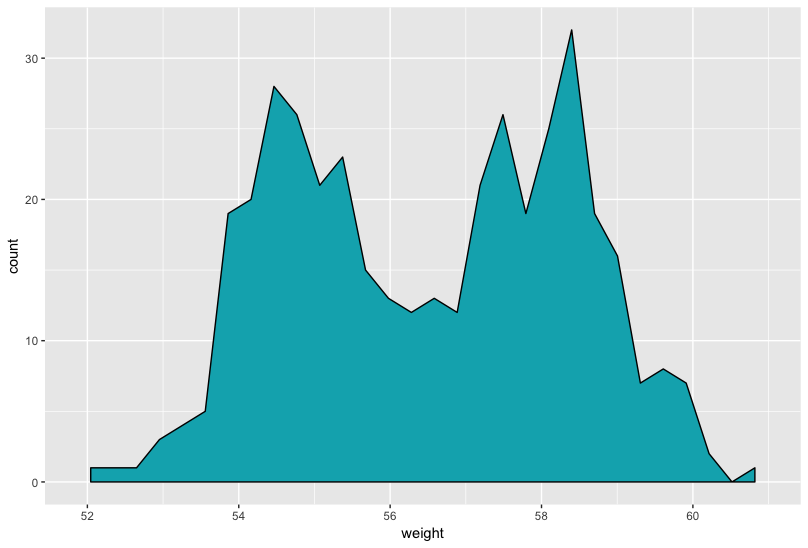
\includegraphics[scale=0.45]{ilu/bg1.png}\end{center}\end{figure}

\textit{a + geom\_area()} will not get right result, object \textit{y} not found. Use stat to specify the count as y.\newline
Note that, by default \textit{y} axis corresponds to the count of weight values. If you want to change the plot in order to have the density on y axis, the R code would be as follow.
\begin{lstlisting}[language=html]
> a + geom\_area(aes(y = ..density..), stat = "bin")
\end{lstlisting}

\begin{figure}[H]\begin{center}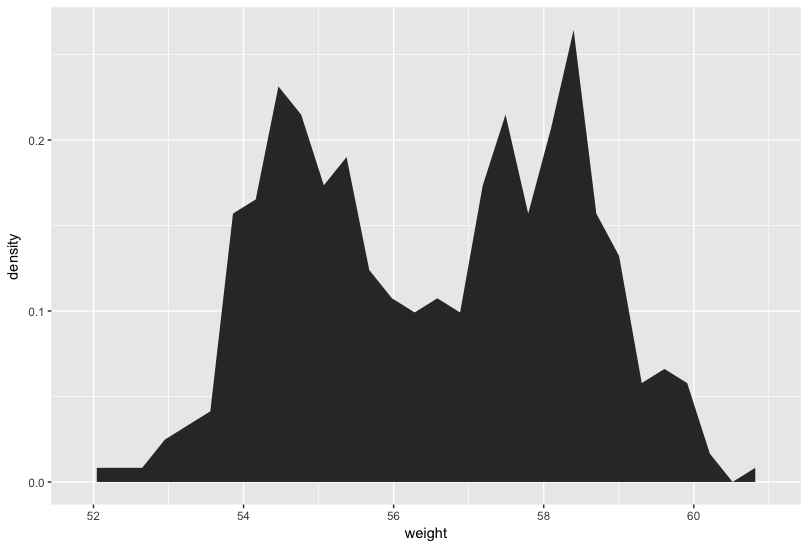
\includegraphics[scale=0.45]{ilu/bg2.png}\end{center}\end{figure}
\begin{lstlisting}[language=html]
> data("diamonds")
> diamonds <- as_data_frame(diamonds)
> diamonds
# A tibble: 53,940 x 10
   carat       cut color clarity depth table price     x     y     z
   <dbl>     <ord> <ord>   <ord> <dbl> <dbl> <int> <dbl> <dbl> <dbl>
 1  0.23     Ideal     E     SI2  61.5    55   326  3.95  3.98  2.43
 2  0.21   Premium     E     SI1  59.8    61   326  3.89  3.84  2.31
 3  0.23      Good     E     VS1  56.9    65   327  4.05  4.07  2.31
 4  0.29   Premium     I     VS2  62.4    58   334  4.20  4.23  2.63
 5  0.31      Good     J     SI2  63.3    58   335  4.34  4.35  2.75
 6  0.24 Very Good     J    VVS2  62.8    57   336  3.94  3.96  2.48
 7  0.24 Very Good     I    VVS1  62.3    57   336  3.95  3.98  2.47
 8  0.26 Very Good     H     SI1  61.9    55   337  4.07  4.11  2.53
 9  0.22      Fair     E     VS2  65.1    61   337  3.87  3.78  2.49
10  0.23 Very Good     H     VS1  59.4    61   338  4.00  4.05  2.39
# ... with 53,930 more rows
\end{lstlisting}
\begin{lstlisting}[language=html]
> p <- ggplot(diamonds, aes(x = price, fill = cut))
# Bar plot
> p + geom_bar(stat = "bin")
\end{lstlisting}
\begin{figure}[H]\begin{center}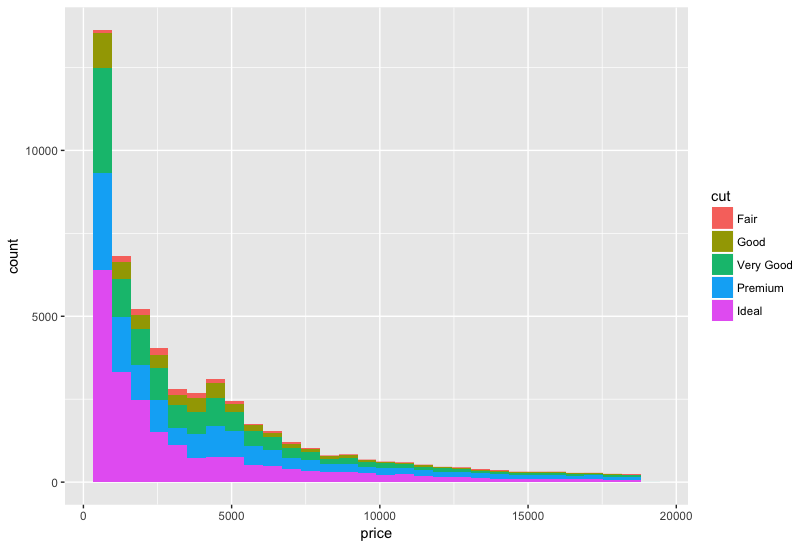
\includegraphics[scale=0.45]{ilu/bg3.png}\end{center}\end{figure}
\begin{lstlisting}[language=html]
# Area plot
> p + geom_area(stat = "bin")
\end{lstlisting}
\begin{figure}[H]\begin{center}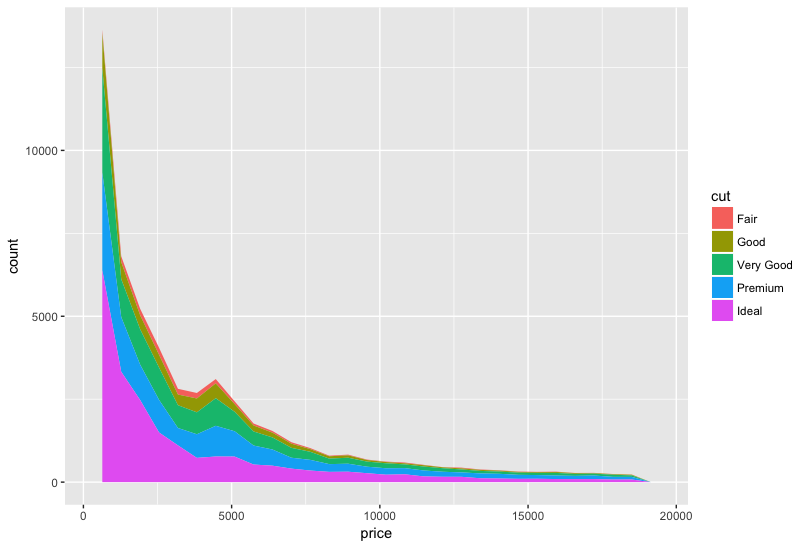
\includegraphics[scale=0.45]{ilu/bg4.png}\end{center}\end{figure}

\subsection{Density Plots}
\textbf{alpha, color, fill, linetype, size}
\begin{itemize}
  \item scale\_color\_manual(), scale\_fill\_manual()
  \item scale\_color\_brewer(), scale\_fill\_brewer() RColor-Brewer
  \item scale\_color\_grey(), scale\_fill\_grey()
\end{itemize}

\begin{lstlisting}[language=html]
# Basic plots
> a + geom_density()
\end{lstlisting}

\begin{figure}[H]\begin{center}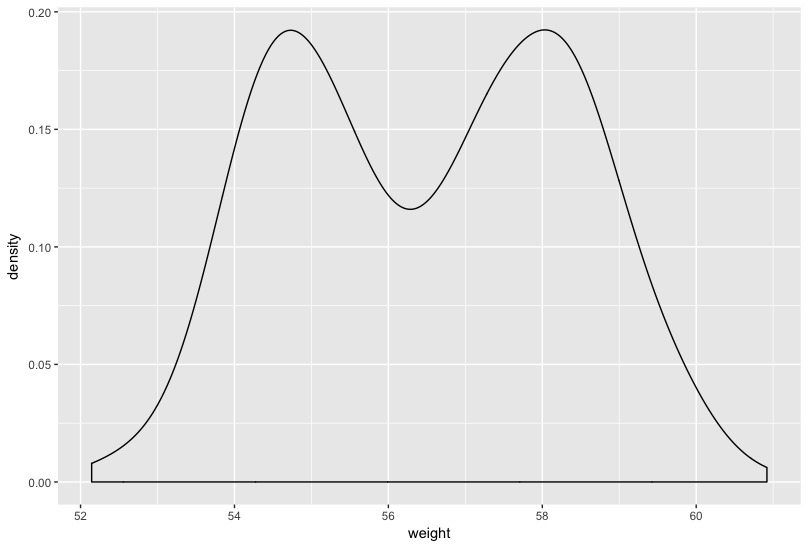
\includegraphics[scale=0.45]{ilu/bg5.png}\end{center}\end{figure}
\begin{lstlisting}[language=html]
# Add color and mean xintercept and median xintercept
> a + geom_density(color = "black", fill = "gray") + geom_vline(aes(xintercept = mean(weight)), color = "#FC4E08", linetype = "dashed", size = 1) + geom_vline(aes(xintercept = median(weight)), color = "blue", linetype = 4, size = 1)
\end{lstlisting}
\begin{figure}[H]\begin{center}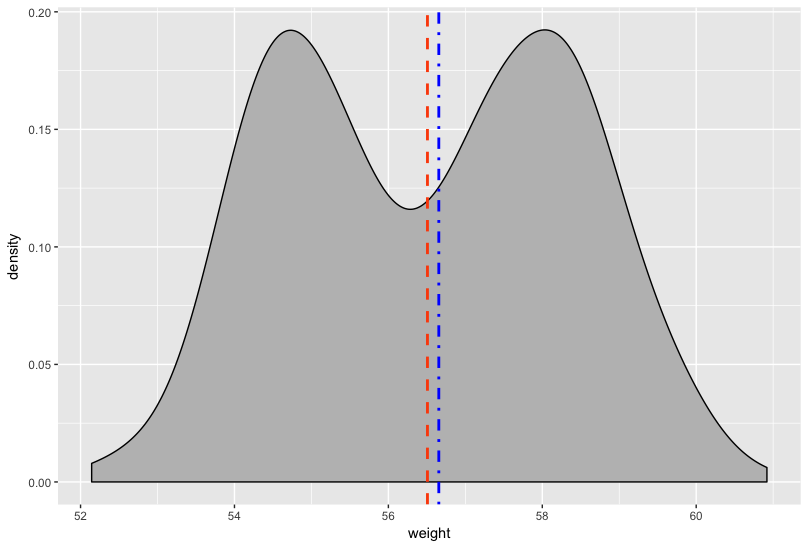
\includegraphics[scale=0.45]{ilu/bg6.png}\end{center}\end{figure}
\begin{lstlisting}[language=html]
# Change color by group
> a + geom_density(aes(fill = sex), alpha = 0.4)
\end{lstlisting}
\begin{figure}[H]\begin{center}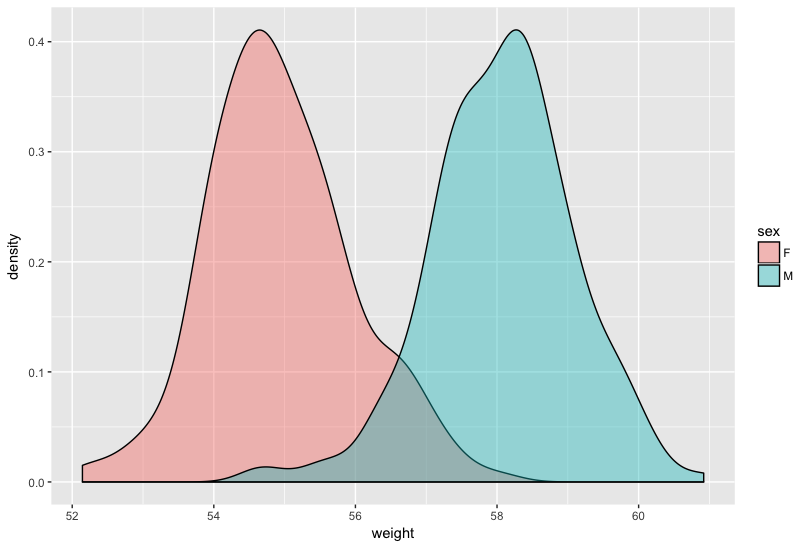
\includegraphics[scale=0.45]{ilu/bg7.png}\end{center}\end{figure}
\begin{lstlisting}[language=html]
# Add mean lines and color by sex
> a + geom_density(aes(fill = sex), alpha = 0.4) + geom_vline(data = mu, aes(xintercept = grp.mean, color = sex), linetype = "dashed")
\end{lstlisting}
\begin{figure}[H]\begin{center}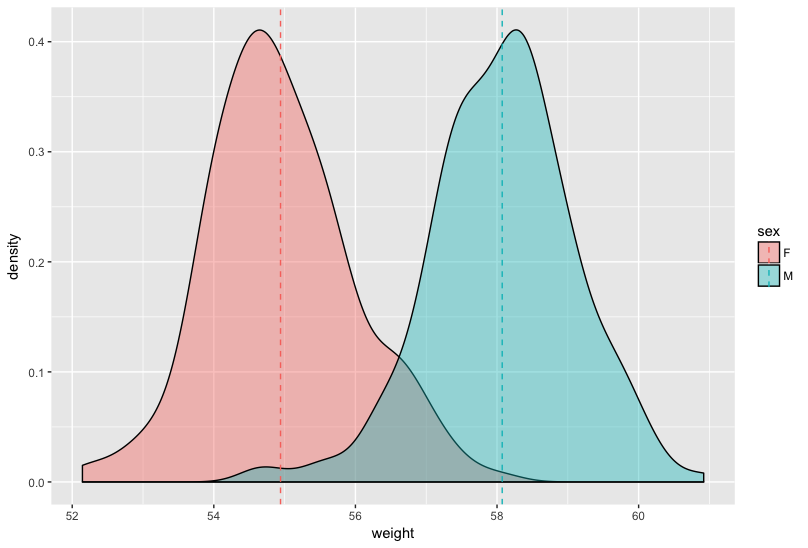
\includegraphics[scale=0.45]{ilu/bg8.png}\end{center}\end{figure}
\begin{lstlisting}[language=html]
# Change manually 
# change line manually
> a2 <- a + geom_density(aes(color = sex)) + geom_vline(data = mu, aes(xintercept = grp.mean, color = sex), linetype = "dashed") + theme_minimal()
> a2 + scale_color_manual(values = c("#999999", "#E69F00"))
\end{lstlisting}
\begin{figure}[H]\begin{center}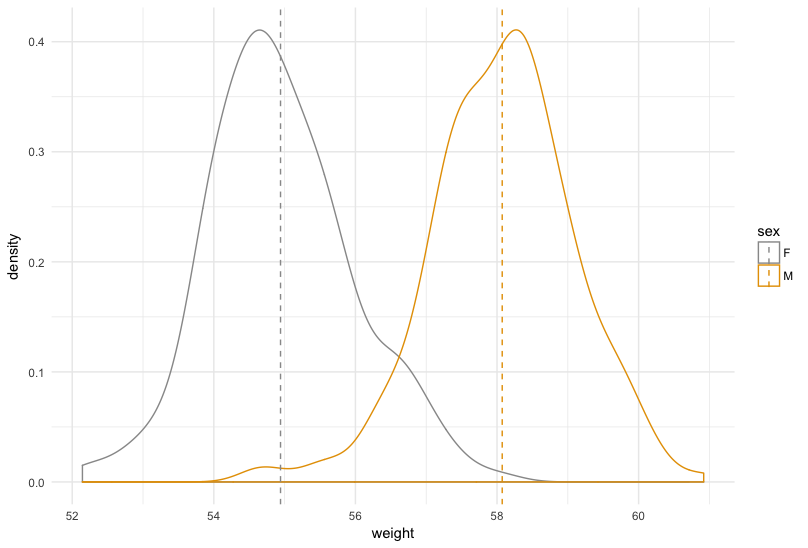
\includegraphics[scale=0.45]{ilu/bg9.png}\end{center}\end{figure}
\begin{lstlisting}[language=html]
> a2 + scale_color_brewer(palette = "Paired")
\end{lstlisting}
\begin{figure}[H]\begin{center}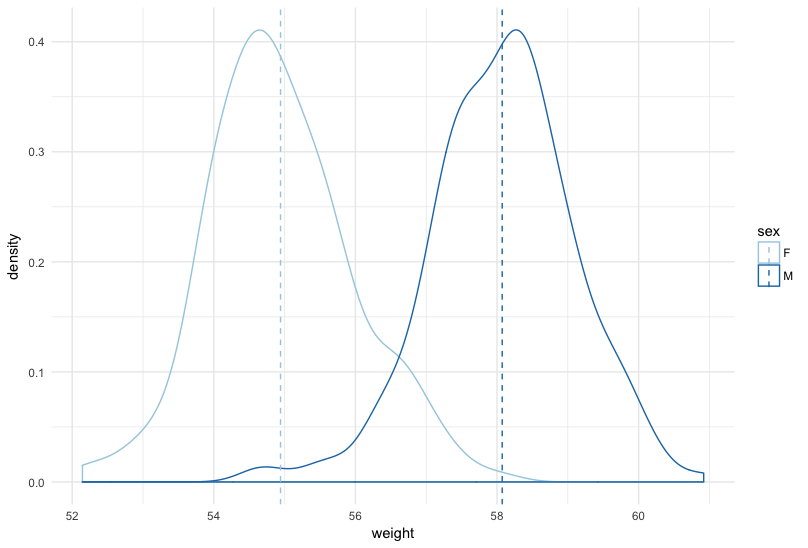
\includegraphics[scale=0.45]{ilu/bg10.png}\end{center}\end{figure}
\begin{lstlisting}[language=html]
> a2 + scale_color_grey()
\end{lstlisting}
\begin{figure}[H]\begin{center}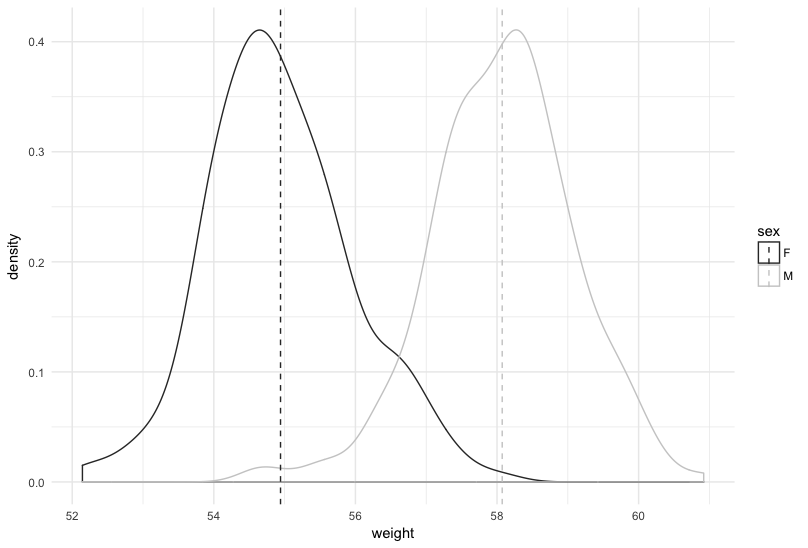
\includegraphics[scale=0.45]{ilu/bg11.png}\end{center}\end{figure}
\begin{lstlisting}[language=html]
# Change fill\footnote{remplissage} manually
> a3 <- a + geom_density(aes(fill = sex), alpha = 0.4) + theme_minimal()
> a3 + scale_fill_manual(values = c("#999999", "#E69F00"))
\end{lstlisting}
\begin{figure}[H]\begin{center}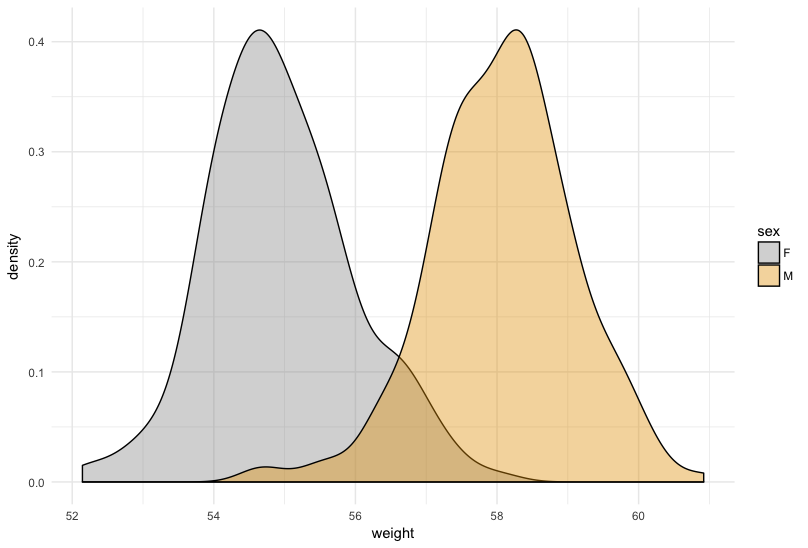
\includegraphics[scale=0.45]{ilu/bg12.png}\end{center}\end{figure}
\begin{lstlisting}[language=html]
> a3 + scale_fill_brewer(palette = "Dark2")
\end{lstlisting}
\begin{figure}[H]\begin{center}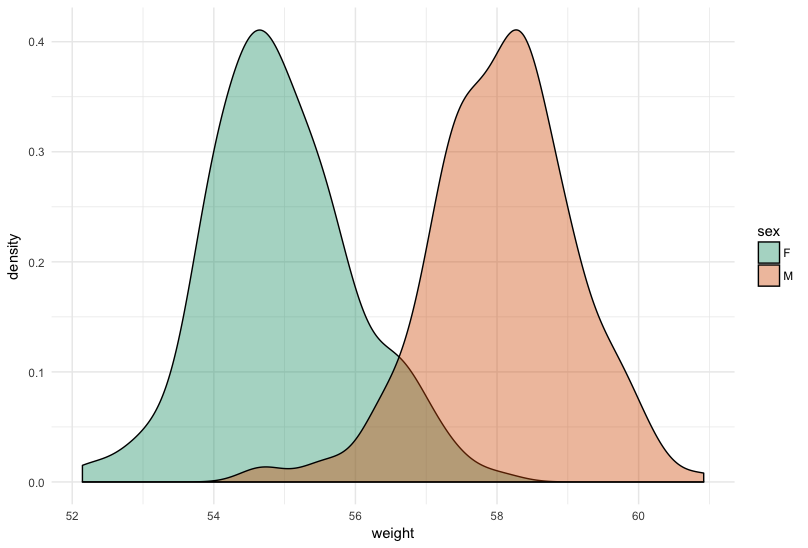
\includegraphics[scale=0.45]{ilu/bg13.png}\end{center}\end{figure}
\begin{lstlisting}[language=html]
> a3 + scale_fill_grey()
\end{lstlisting}
\begin{figure}[H]\begin{center}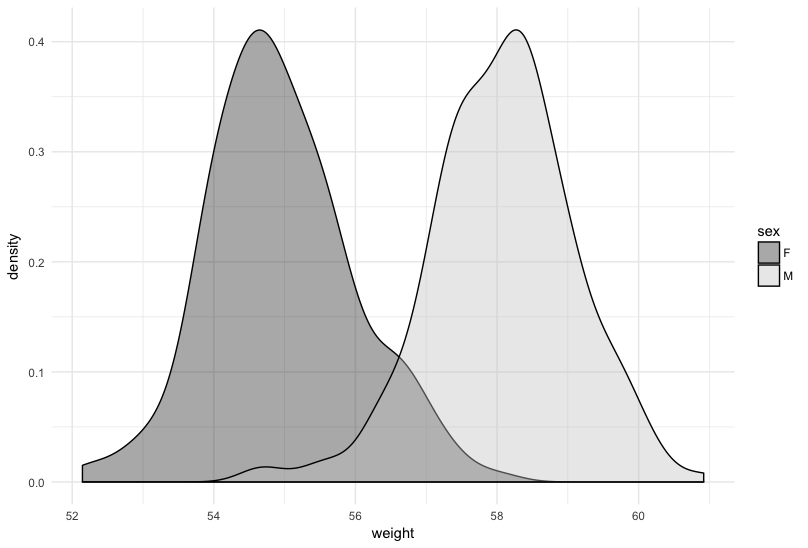
\includegraphics[scale=0.45]{ilu/bg14.png}\end{center}\end{figure}

\subsection{Histogram Plots}
\textbf{identity(position\_identity()), stack(position\_stack()), dodge(position\_dodge()); Default values is "stack"}\newline
\\
\textbf{alpha, color, fill, linetype, size}
\begin{lstlisting}[language=html]
# Basic plot
> a + geom_histogram()
\end{lstlisting}
\begin{figure}[H]\begin{center}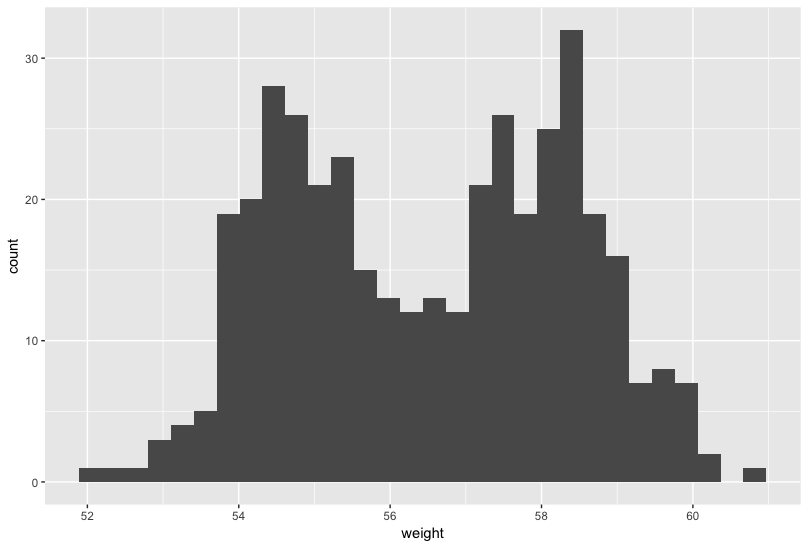
\includegraphics[scale=0.45]{ilu/bg15.png}\end{center}\end{figure}
\begin{lstlisting}[language=html]
> a + geom_histogram(bins = 50)
\end{lstlisting}
\begin{figure}[H]\begin{center}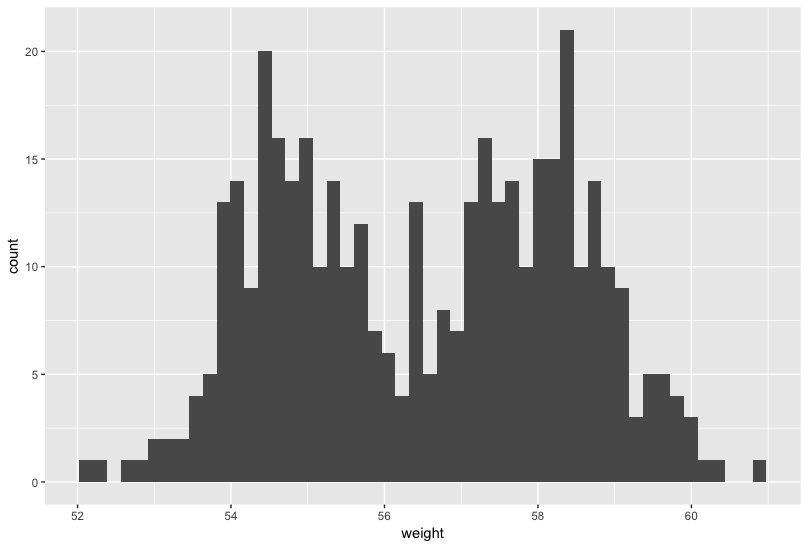
\includegraphics[scale=0.45]{ilu/bg16.png}\end{center}\end{figure}
Note that by default, stat\_bin uses 30 bins - this might not be good default. You can change the number of bins (\textit{e.g.}: bins = 50 or the bin width \textit{e.g.}: binwidth = 0.5.
\begin{lstlisting}[language=html]
> a + geom_histogram(bins = 50, color = "black", fill = "grey") + geom_vline(aes(xintercept = mean(weight)), color = "#FC4E07", linetype = "dashed", size = 1) + theme_minimal()
\end{lstlisting}
\begin{figure}[H]\begin{center}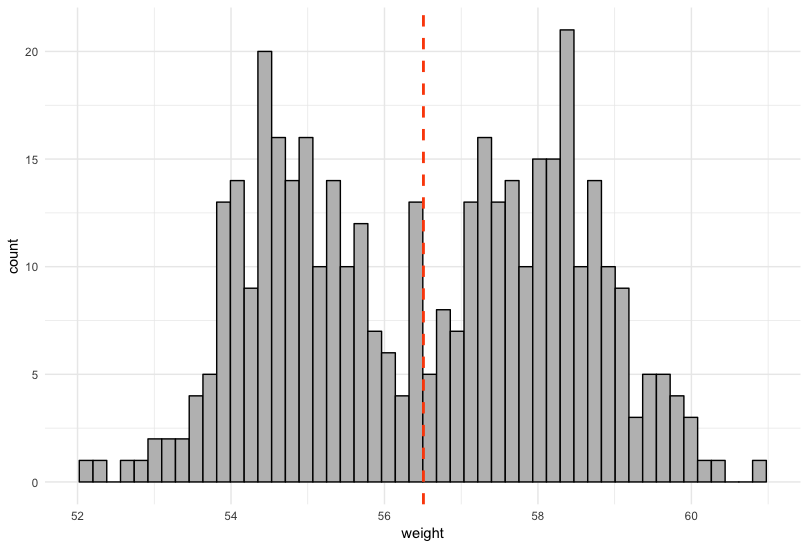
\includegraphics[scale=0.45]{ilu/bg17.png}\end{center}\end{figure}
\begin{lstlisting}[language=html]
> a + geom_histogram(aes(y = ..density..), bins = 50)
\end{lstlisting}
\begin{figure}[H]\begin{center}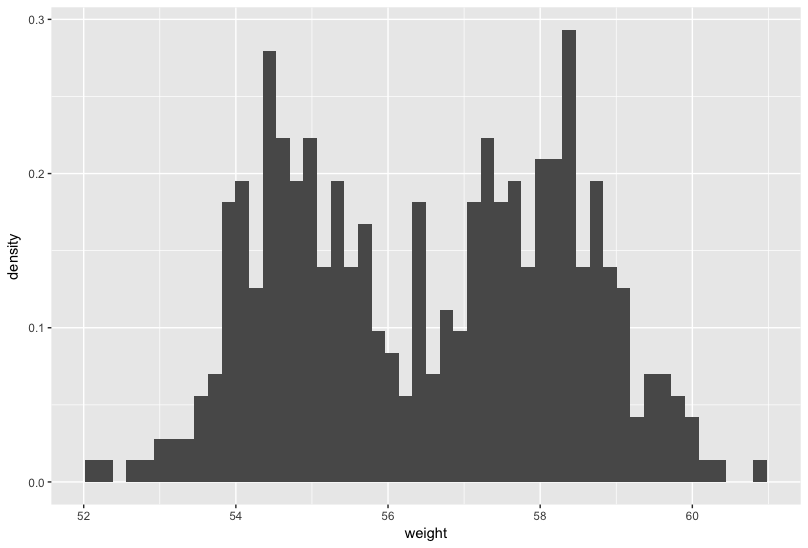
\includegraphics[scale=0.45]{ilu/bg18.png}\end{center}\end{figure}
\begin{lstlisting}[language=html]
# Change color by sex
> a + geom_histogram(aes(color = sex), fill = "white", bins = 50) + theme_minimal()
\end{lstlisting}
\begin{figure}[H]\begin{center}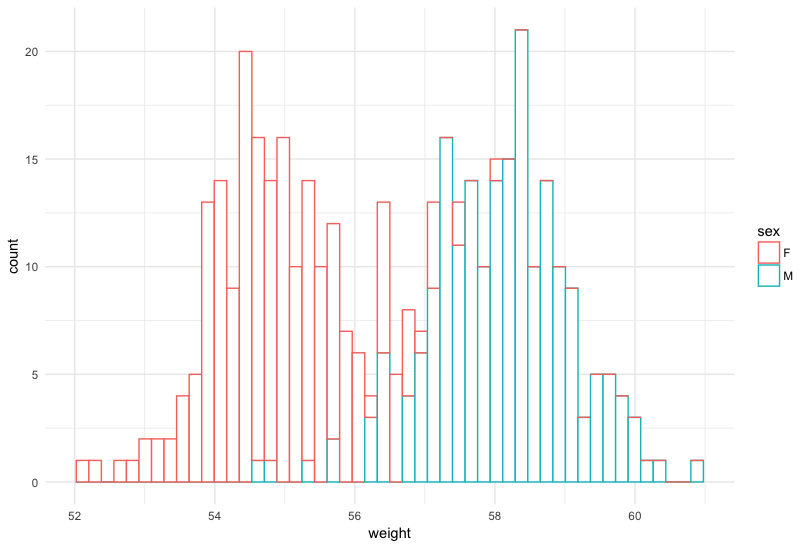
\includegraphics[scale=0.45]{ilu/bg19.png}\end{center}\end{figure}
\begin{lstlisting}[language=html]
# Position adjustment "identity"(overlaid)
> a + geom_histogram(aes(color = sex), fill = "white", bins = 50, alpha = 0.6, position = "identity")
\end{lstlisting}
\begin{figure}[H]\begin{center}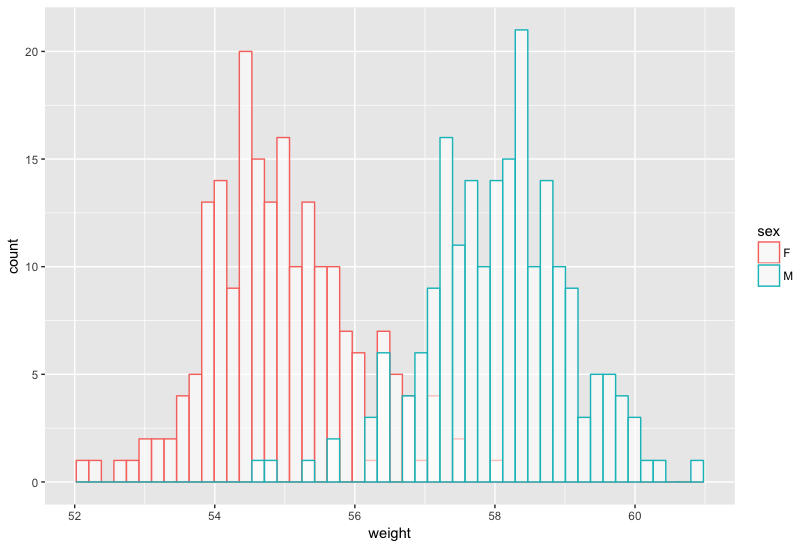
\includegraphics[scale=0.45]{ilu/bg20.png}\end{center}\end{figure}
\begin{lstlisting}[language=html]
# Position adjustment "dodge" (Interleaved)
# Add mean lines and color by sex
> a + geom_histogram(aes(color = sex), fill = "white", alpha = 0.6, position = "dodge", bins = 50) + geom_vline(aes(xintercept = mean(weight)), linetype = "dashed")
\end{lstlisting}
\begin{figure}[H]\begin{center}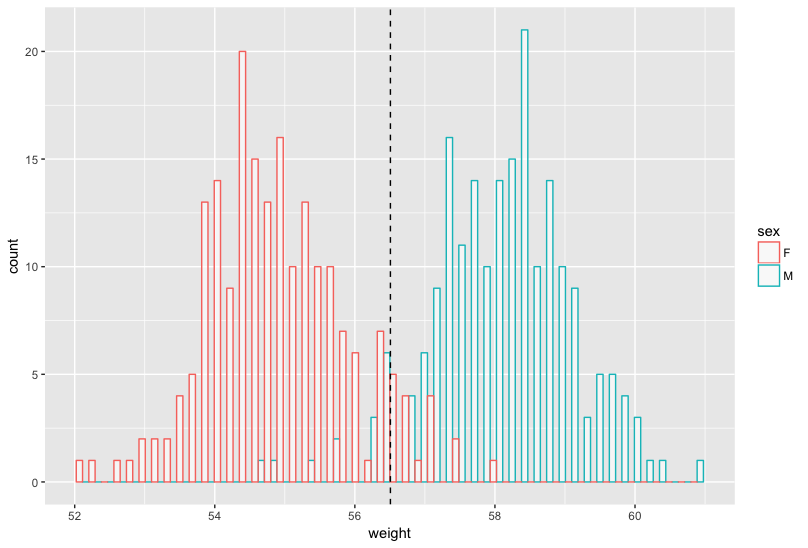
\includegraphics[scale=0.45]{ilu/bg21.png}\end{center}\end{figure}
\begin{lstlisting}[language=html]
# Change fill, color manually
# Change outline color manually
> a + geom_histogram(aes(color = sex), fill = "white", alpha = 0.4, position = "identity", bins = 50) + scale_color_manual(values = c("#00AFBB","#E7B800"))
\end{lstlisting}
\begin{figure}[H]\begin{center}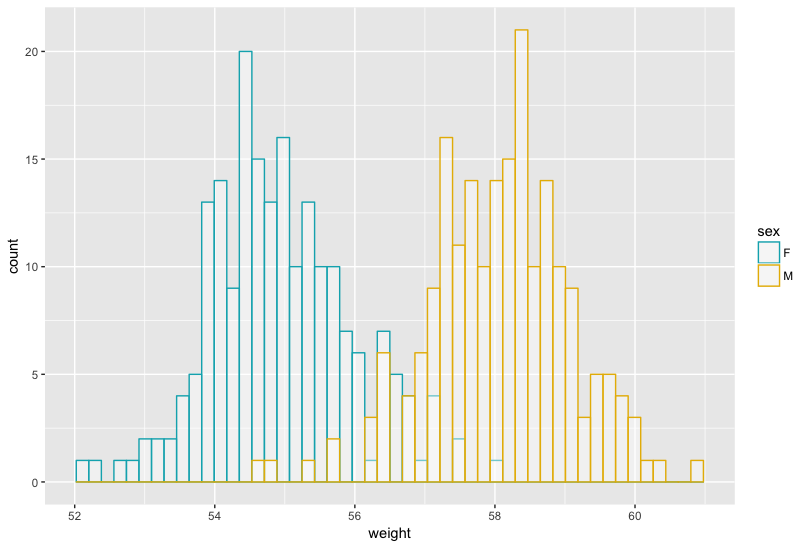
\includegraphics[scale=0.45]{ilu/bg22.png}\end{center}\end{figure}
\begin{lstlisting}[language=html]
# Change fill and outline color manually
# a + geom_histogram(aes(color = sex), fill = "white", alpha =0.4, position = "identity", bins = 50) + scale_fill_manual(values = c("#00AFBB", "#E7B800")) + scale_color_manual(values = c("#00AFBB", "#E7B800")) 
# wrong command, I have to assign fill first by group
> a + geom_histogram(aes(color = sex, fill = sex), alpha =0.4, position = "identity", bins = 50) + scale_fill_manual(values = c("#00AFBB", "#E7B800")) + scale_color_manual(values = c("#00AFBB", "#E7B800"))
\end{lstlisting}
\begin{figure}[H]\begin{center}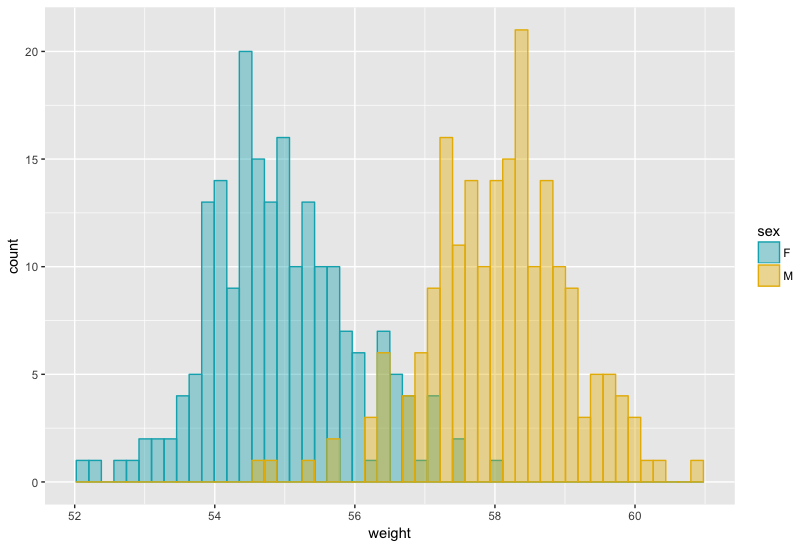
\includegraphics[scale=0.45]{ilu/bg23.png}\end{center}\end{figure}
\begin{lstlisting}[language=html]
## Combine Histogram and Density Plots
# Plot histogram with density values on y-axis(instead of count values).
# Add density plot with transparent density plot
# Histogram with density plot

> a + geom_histogram(aes(y = ..density..),color = "black", fill = "white") + geom_density(alpha = 0.2, fill = "#FF6666") + theme_minimal()
\end{lstlisting}
\begin{figure}[H]\begin{center}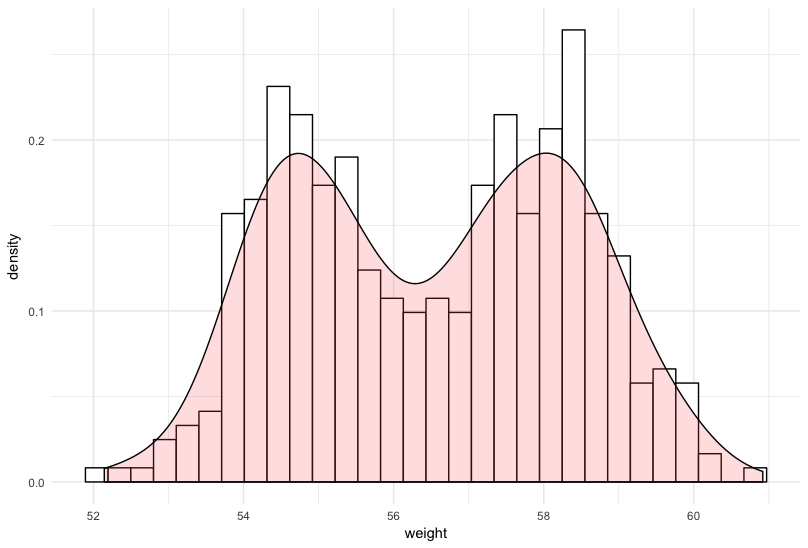
\includegraphics[scale=0.45]{ilu/bg24.png}\end{center}\end{figure}
\begin{lstlisting}[language=html]
# Color by groups
> a + geom_histogram(aes(y = ..density.., color = sex, fill = sex),  alpha = 0.4, position = "identity") + geom_density(aes(color = sex), size =1)
\end{lstlisting}
\begin{figure}[H]\begin{center}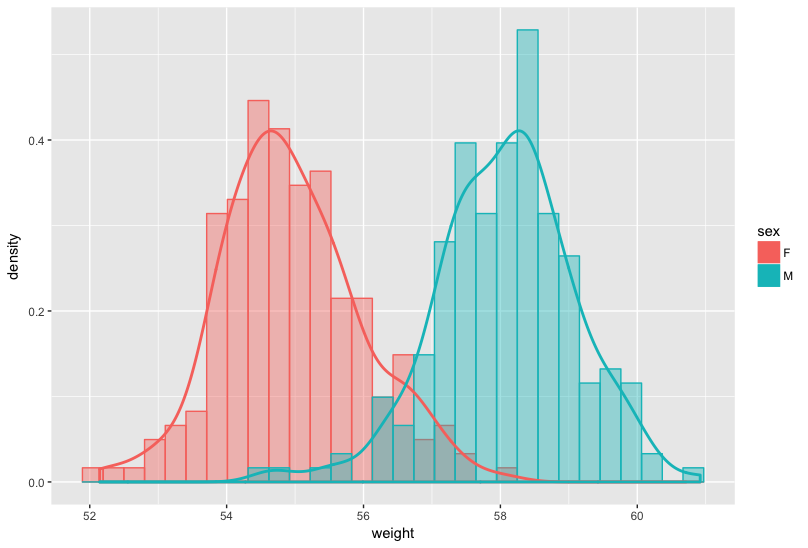
\includegraphics[scale=0.45]{ilu/bg25.png}\end{center}\end{figure}
\subsection{Frequency Polygon}
Very close to histogram plots
\begin{itemize}
  \item Histogram use bars
  \item Frequency polygons use lines.
\end{itemize}
\textbf{alpha, color, linetype, size}
\begin{lstlisting}[language=html]
# Basic plot
> a + geom_freqpoly(bins = 30) + theme_minimal()
\end{lstlisting}
\begin{figure}[H]\begin{center}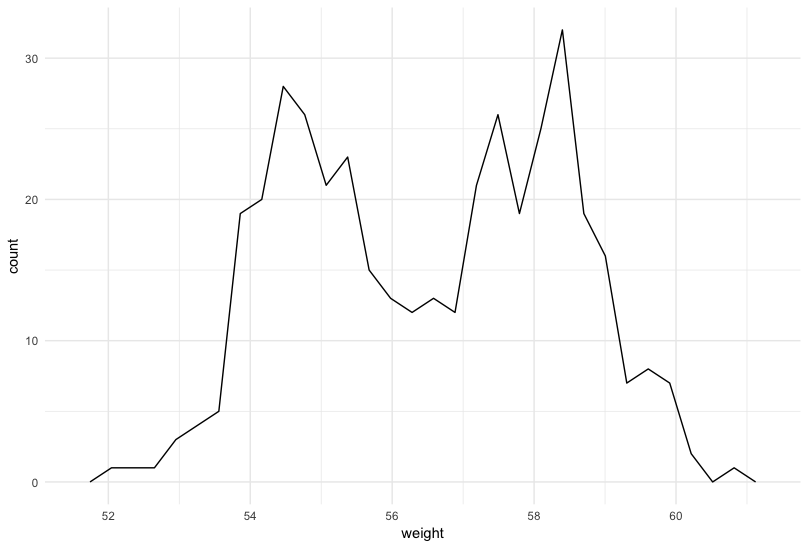
\includegraphics[scale=0.45]{ilu/bg26.png}\end{center}\end{figure}
\begin{lstlisting}[language=html]
# Change color and linetype by sex
# Use custom color palettes
a + geom_freqpoly(aes(color = sex, linetype = sex), bins = 30 ) +  scale_color_manual(values = c("#999999", "#E69F00"))+theme_minimal()
\end{lstlisting}
\begin{figure}[H]\begin{center}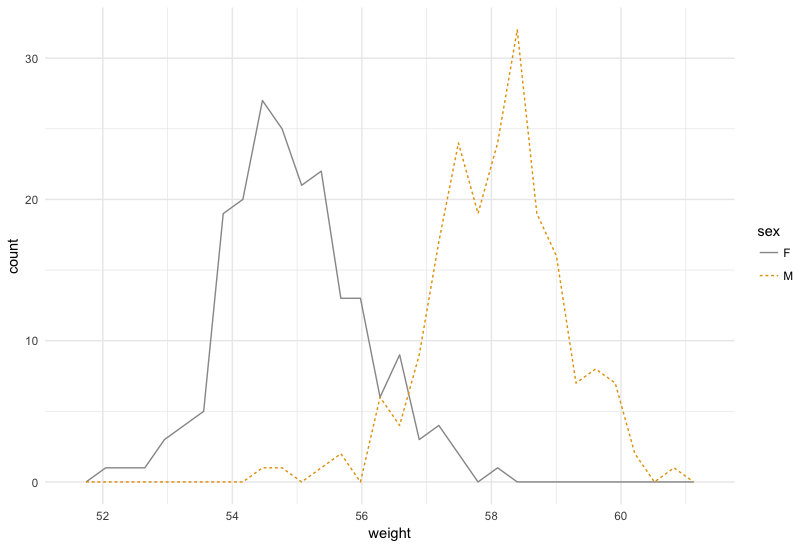
\includegraphics[scale=0.45]{ilu/bg27.png}\end{center}\end{figure}
\begin{lstlisting}[language=html]
# y density
> a + geom_freqpoly(aes(y = ..density.., color = sex, linetype = sex), bins = 30 ) +  scale_color_manual(values = c("#999999", "#E69F00"))+theme_minimal()
\end{lstlisting}
\begin{figure}[H]\begin{center}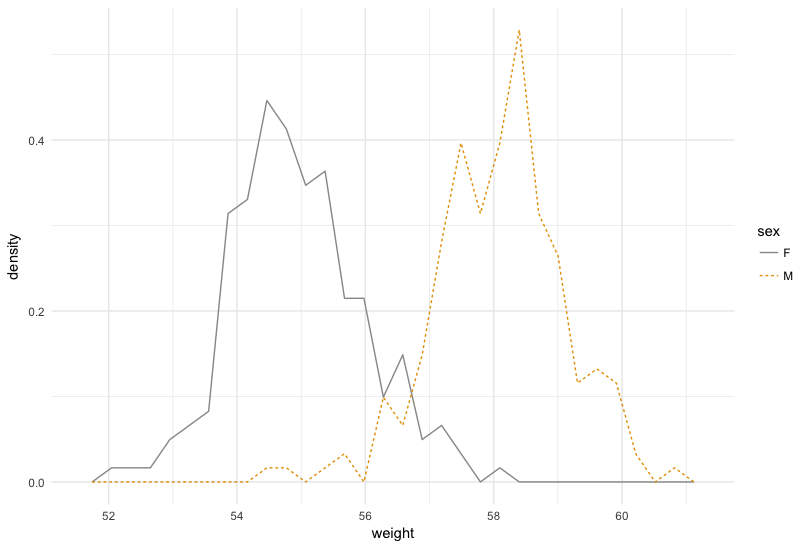
\includegraphics[scale=0.45]{ilu/bg28.png}\end{center}\end{figure}
\subsection{Dot Plots for One Variable}
Not suitable for one variable, it?s ugly.
\begin{lstlisting}[language=html]
> a + geom_dotplot(aes(fill = sex))
\end{lstlisting}
\begin{figure}[H]\begin{center}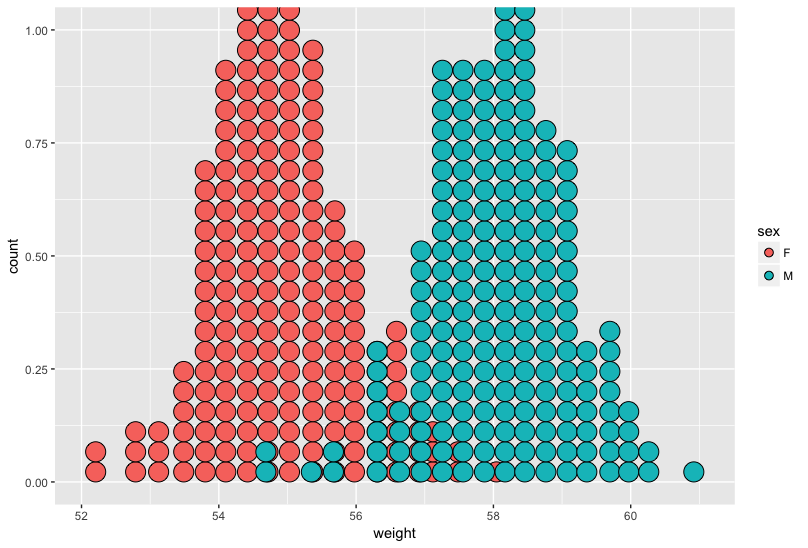
\includegraphics[scale=0.45]{ilu/bg29.png}\end{center}\end{figure}
\subsection{ECDF Plots}
Empirical Cumulative Density Function\newline
\\
\textbf{alpha, color, linetype, size}
\begin{lstlisting}[language=html]
> a + stat\_ecdf(geom = "point")
\end{lstlisting}
\begin{figure}[H]\begin{center}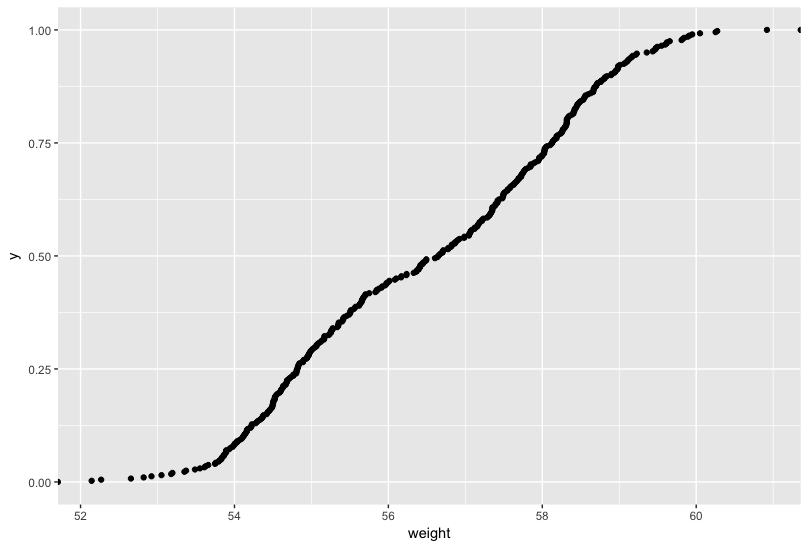
\includegraphics[scale=0.45]{ilu/bg30.png}\end{center}\end{figure}
\begin{lstlisting}[language=html]
> a + stat\_ecdf(geom = "step")
\end{lstlisting}
\begin{figure}[H]\begin{center}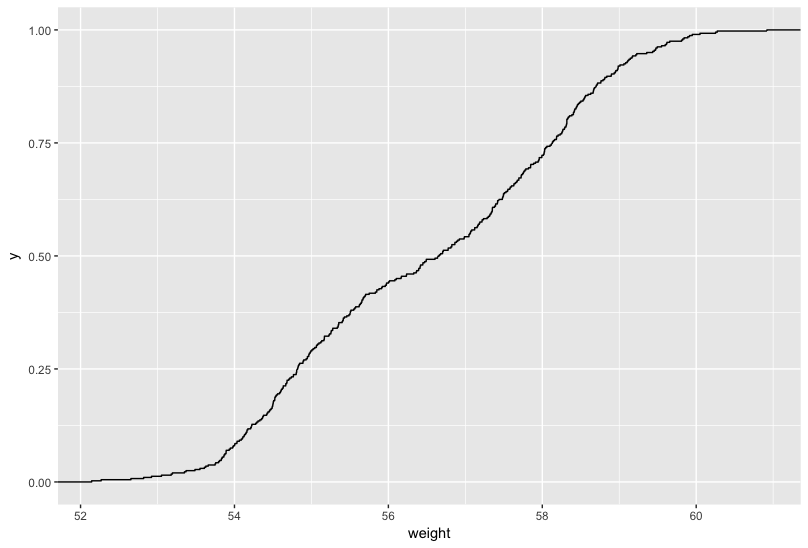
\includegraphics[scale=0.45]{ilu/bg31.png}\end{center}\end{figure}
\subsection{QQ Plots}
Quantile - Quantie plots to chech whether a given data follows normal distribution.\newline
\\
\textbf{alpha, color, shape, size}
\begin{lstlisting}[language=html]
> data(mtcars)
> mtcars <- as_data_frame(mtcars)
> mtcars
# A tibble: 32 x 11
     mpg   cyl  disp    hp  drat    wt  qsec    vs    am  gear  carb
 * <dbl> <dbl> <dbl> <dbl> <dbl> <dbl> <dbl> <dbl> <dbl> <dbl> <dbl>
 1  21.0     6 160.0   110  3.90 2.620 16.46     0     1     4     4
 2  21.0     6 160.0   110  3.90 2.875 17.02     0     1     4     4
 3  22.8     4 108.0    93  3.85 2.320 18.61     1     1     4     1
 4  21.4     6 258.0   110  3.08 3.215 19.44     1     0     3     1
 5  18.7     8 360.0   175  3.15 3.440 17.02     0     0     3     2
 6  18.1     6 225.0   105  2.76 3.460 20.22     1     0     3     1
 7  14.3     8 360.0   245  3.21 3.570 15.84     0     0     3     4
 8  24.4     4 146.7    62  3.69 3.190 20.00     1     0     4     2
 9  22.8     4 140.8    95  3.92 3.150 22.90     1     0     4     2
10  19.2     6 167.6   123  3.92 3.440 18.30     1     0     4     4
# ... with 22 more rows
\end{lstlisting}
\begin{lstlisting}[language=html]
> mtcars <- mutate(mtcars, cyl = as.factor(cyl))
> mtcars
# A tibble: 32 x 11
     mpg    cyl  disp    hp  drat    wt  qsec    vs    am  gear  carb
   <dbl> <fctr> <dbl> <dbl> <dbl> <dbl> <dbl> <dbl> <dbl> <dbl> <dbl>
 1  21.0      6 160.0   110  3.90 2.620 16.46     0     1     4     4
 2  21.0      6 160.0   110  3.90 2.875 17.02     0     1     4     4
 3  22.8      4 108.0    93  3.85 2.320 18.61     1     1     4     1
 4  21.4      6 258.0   110  3.08 3.215 19.44     1     0     3     1
 5  18.7      8 360.0   175  3.15 3.440 17.02     0     0     3     2
 6  18.1      6 225.0   105  2.76 3.460 20.22     1     0     3     1
 7  14.3      8 360.0   245  3.21 3.570 15.84     0     0     3     4
 8  24.4      4 146.7    62  3.69 3.190 20.00     1     0     4     2
 9  22.8      4 140.8    95  3.92 3.150 22.90     1     0     4     2
10  19.2      6 167.6   123  3.92 3.440 18.30     1     0     4     4
# ... with 22 more rows
\end{lstlisting}
\begin{lstlisting}[language=html]
> p <- ggplot(mtcars, aes(sample = mpg))
# Basic plot
> p + stat\_qq()
\end{lstlisting}
\begin{figure}[H]\begin{center}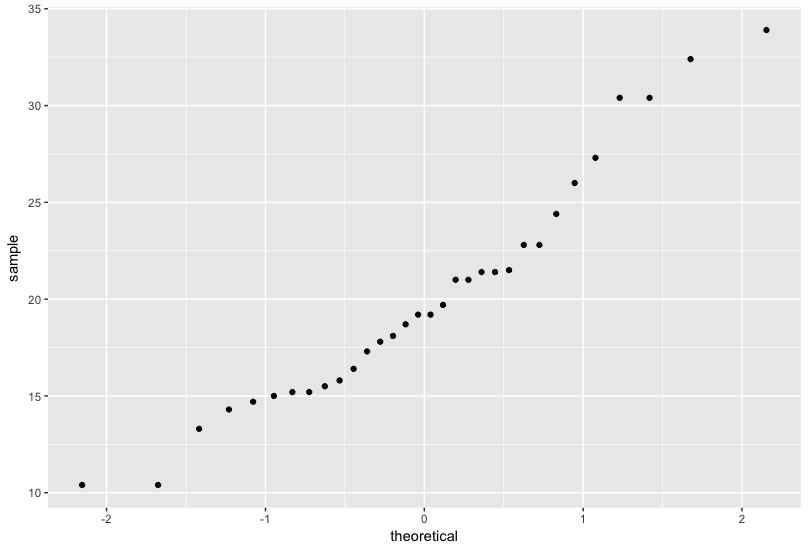
\includegraphics[scale=0.45]{ilu/bg32.png}\end{center}\end{figure}
\begin{lstlisting}[language=html]
# Change point shapes by groups
# Use custom color palettes
> p + stat\_qq(aes(shape = cyl, color = cyl)) + scale_color_manual(values = c("#00AFBB", "#E7B800", "#FC4E07"))
\end{lstlisting}
\begin{figure}[H]\begin{center}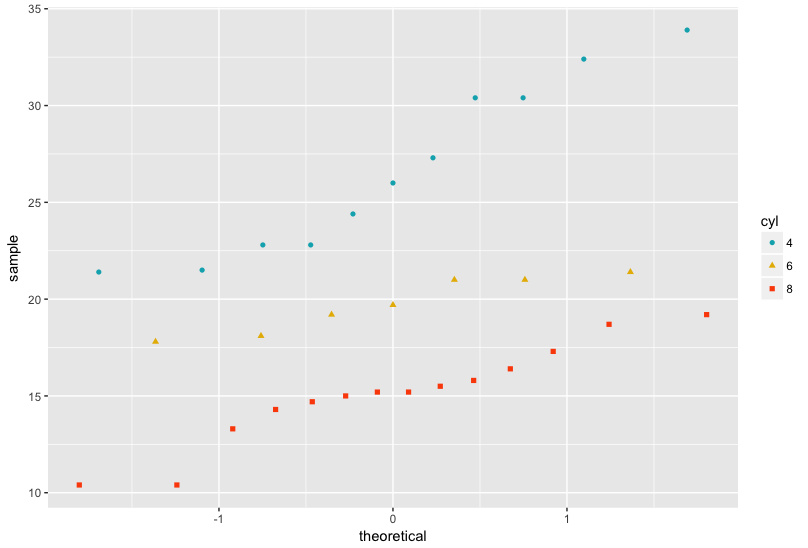
\includegraphics[scale=0.45]{ilu/bg33.png}\end{center}\end{figure}

\subsection{Bar Plots of Counts}
For one discrete variable\newline
\\
\textbf{alpha, color, fill, linetype, size}
\begin{lstlisting}[language=html]
> data(mpg)
> mpg <- as_data_frame(mpg)
> mpg
# A tibble: 234 x 11
   manufacturer      model displ  year   cyl      trans   drv   cty   hwy
          <chr>      <chr> <dbl> <int> <int>      <chr> <chr> <int> <int>
 1         audi         a4   1.8  1999     4   auto(l5)     f    18    29
 2         audi         a4   1.8  1999     4 manual(m5)     f    21    29
 3         audi         a4   2.0  2008     4 manual(m6)     f    20    31
 4         audi         a4   2.0  2008     4   auto(av)     f    21    30
 5         audi         a4   2.8  1999     6   auto(l5)     f    16    26
 6         audi         a4   2.8  1999     6 manual(m5)     f    18    26
 7         audi         a4   3.1  2008     6   auto(av)     f    18    27
 8         audi a4 quattro   1.8  1999     4 manual(m5)     4    18    26
 9         audi a4 quattro   1.8  1999     4   auto(l5)     4    16    25
10         audi a4 quattro   2.0  2008     4 manual(m6)     4    20    28
# ... with 224 more rows, and 2 more variables: fl <chr>, class <chr>
\end{lstlisting}
\begin{lstlisting}[language=html]
> ggplot(mpg, aes(fl)) + geom_bar(fill = "steelblue") + theme_minimal()
\end{lstlisting}
\begin{figure}[H]\begin{center}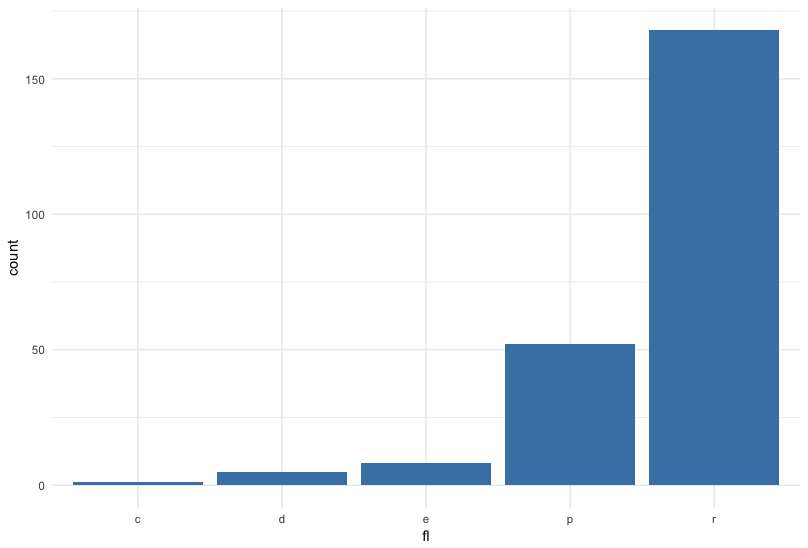
\includegraphics[scale=0.45]{ilu/bg34.png}\end{center}\end{figure}
\section{Plot Two Variables - X \& Y: Both Continuous or Discrete}
\subsection{Scatter plots: Continuous X and Y}
\begin{itemize}
  \item geom\_pint()
  \item geom\_smooth()
  \item geom\_quantile()
  \item geom\_rug()
  \item geom\_jitter()
  \item geom\_text()
\end{itemize}
geom\_point\newline
\textbf{alpha, color, fill, shape, size}
\begin{lstlisting}[language=html]
# Data format
> mtcars
                     mpg cyl  disp  hp drat    wt  qsec vs am gear carb
Mazda RX4           21.0   6 160.0 110 3.90 2.620 16.46  0  1    4    4
Mazda RX4 Wag       21.0   6 160.0 110 3.90 2.875 17.02  0  1    4    4
Datsun 710          22.8   4 108.0  93 3.85 2.320 18.61  1  1    4    1
Hornet 4 Drive      21.4   6 258.0 110 3.08 3.215 19.44  1  0    3    1
Hornet Sportabout   18.7   8 360.0 175 3.15 3.440 17.02  0  0    3    2
Valiant             18.1   6 225.0 105 2.76 3.460 20.22  1  0    3    1
Duster 360          14.3   8 360.0 245 3.21 3.570 15.84  0  0    3    4
Merc 240D           24.4   4 146.7  62 3.69 3.190 20.00  1  0    4    2
Merc 230            22.8   4 140.8  95 3.92 3.150 22.90  1  0    4    2
Merc 280            19.2   6 167.6 123 3.92 3.440 18.30  1  0    4    4
Merc 280C           17.8   6 167.6 123 3.92 3.440 18.90  1  0    4    4
Merc 450SE          16.4   8 275.8 180 3.07 4.070 17.40  0  0    3    3
Merc 450SL          17.3   8 275.8 180 3.07 3.730 17.60  0  0    3    3
Merc 450SLC         15.2   8 275.8 180 3.07 3.780 18.00  0  0    3    3
Cadillac Fleetwood  10.4   8 472.0 205 2.93 5.250 17.98  0  0    3    4
Lincoln Continental 10.4   8 460.0 215 3.00 5.424 17.82  0  0    3    4
Chrysler Imperial   14.7   8 440.0 230 3.23 5.345 17.42  0  0    3    4
Fiat 128            32.4   4  78.7  66 4.08 2.200 19.47  1  1    4    1
Honda Civic         30.4   4  75.7  52 4.93 1.615 18.52  1  1    4    2
Toyota Corolla      33.9   4  71.1  65 4.22 1.835 19.90  1  1    4    1
Toyota Corona       21.5   4 120.1  97 3.70 2.465 20.01  1  0    3    1
Dodge Challenger    15.5   8 318.0 150 2.76 3.520 16.87  0  0    3    2
AMC Javelin         15.2   8 304.0 150 3.15 3.435 17.30  0  0    3    2
Camaro Z28          13.3   8 350.0 245 3.73 3.840 15.41  0  0    3    4
Pontiac Firebird    19.2   8 400.0 175 3.08 3.845 17.05  0  0    3    2
Fiat X1-9           27.3   4  79.0  66 4.08 1.935 18.90  1  1    4    1
Porsche 914-2       26.0   4 120.3  91 4.43 2.140 16.70  0  1    5    2
Lotus Europa        30.4   4  95.1 113 3.77 1.513 16.90  1  1    5    2
Ford Pantera L      15.8   8 351.0 264 4.22 3.170 14.50  0  1    5    4
Ferrari Dino        19.7   6 145.0 175 3.62 2.770 15.50  0  1    5    6
Maserati Bora       15.0   8 301.0 335 3.54 3.570 14.60  0  1    5    8
Volvo 142E          21.4   4 121.0 109 4.11 2.780 18.60  1  1    4    2
\end{lstlisting}
\begin{lstlisting}[language=html]
> b <- ggplot(mtcars, aes(x = wt, y= mpg))
# x weight
# y miles/gallon
#Basic scatter plots
> b + geom_point(color = "#00AFBB")
\end{lstlisting}

\begin{figure}[H]\begin{center}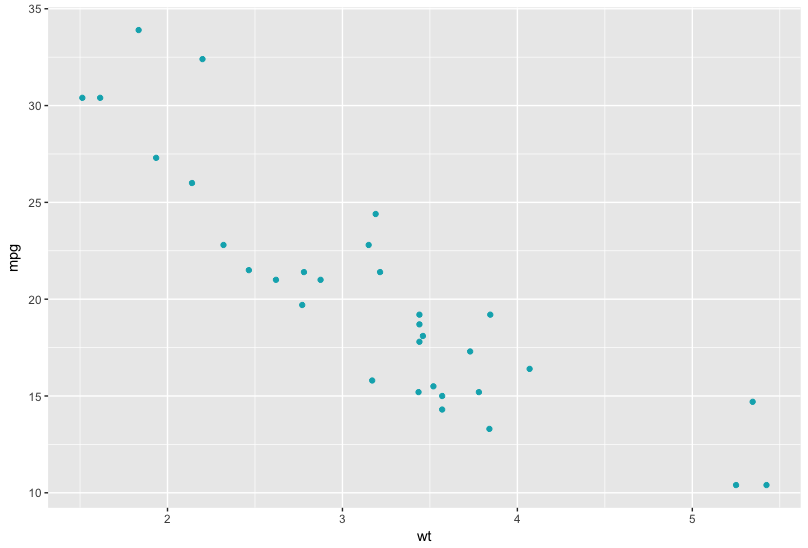
\includegraphics[scale=0.45]{ilu/bg35.png}\end{center}\end{figure}
\begin{lstlisting}[language=html]
# Change the point size, and shape
> b + geom_point(color = "#00AFBB", size = 2, shape = 23)
\end{lstlisting}
\begin{figure}[H]\begin{center}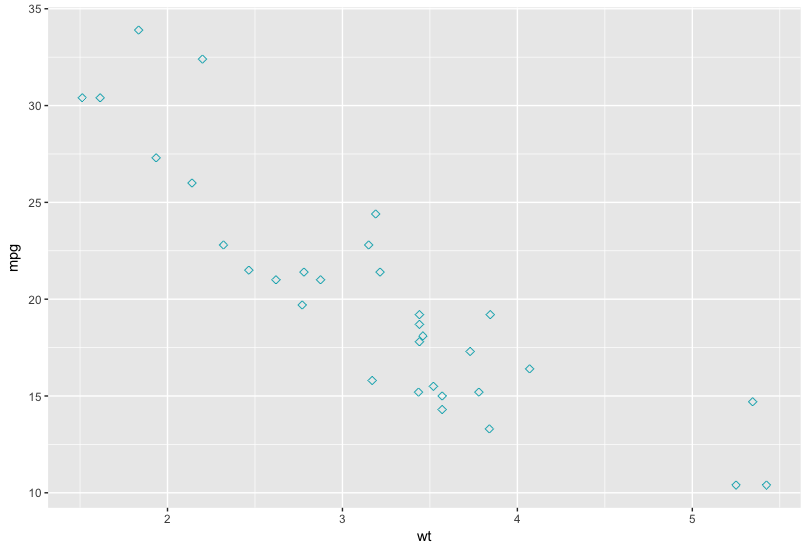
\includegraphics[scale=0.45]{ilu/bg36.png}\end{center}\end{figure}
\begin{lstlisting}[language=html]
# Control point size by continuous variable values
# qsec 1/4 mile time
> b + geom_point(aes(size = qsec), color = "#00AFBB")
\end{lstlisting}
\begin{figure}[H]\begin{center}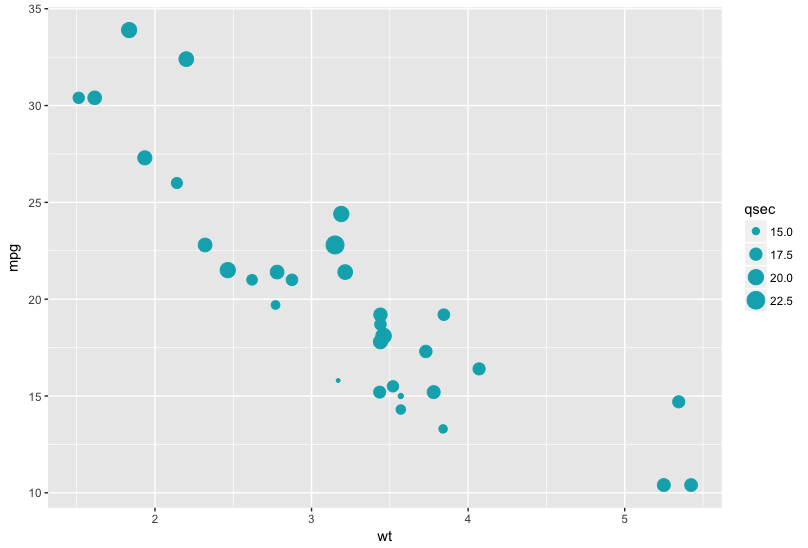
\includegraphics[scale=0.45]{ilu/bg37.png}\end{center}\end{figure}
\begin{lstlisting}[language=html]
# Label text
> b + geom_point() + geom_text(label = rownames(mtcars), nudge_y = 0.8)
\end{lstlisting}
\begin{figure}[H]\begin{center}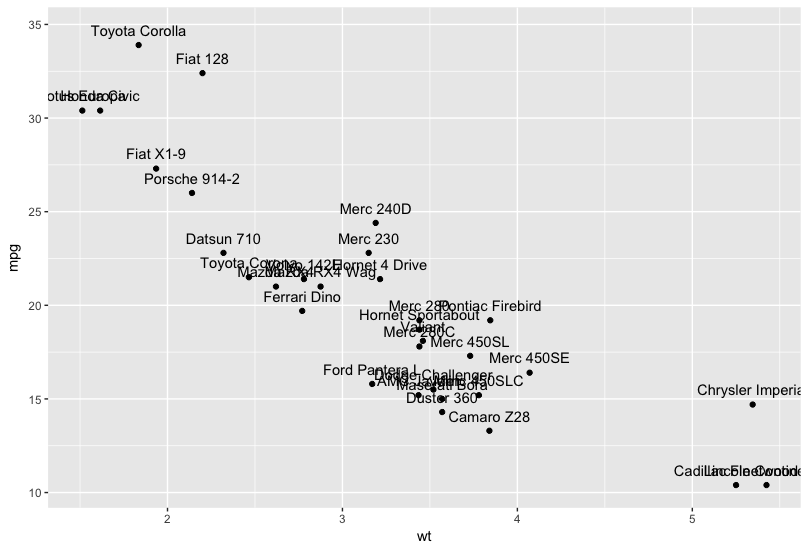
\includegraphics[scale=0.45]{ilu/bg38.png}\end{center}\end{figure}
\begin{lstlisting}[language=html]
# Change shape, color, size automatically
# Change point shape by the level of cyl
> b + geom_point(aes(shape = factor(cyl)))
\end{lstlisting}
\begin{figure}[H]\begin{center}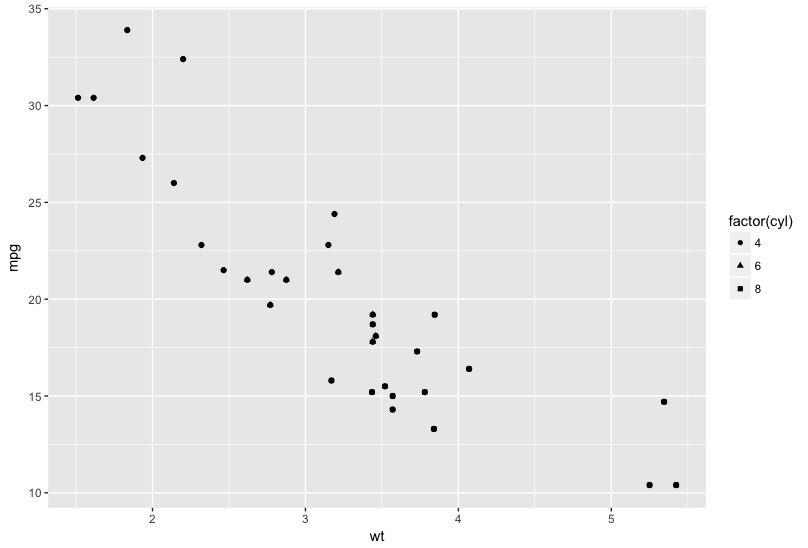
\includegraphics[scale=0.45]{ilu/bg39.png}\end{center}\end{figure}
\begin{lstlisting}[language=html]
# Change point shape and colors
> b + geom_point(aes(color = cyl, shape=factor(cyl)))
\end{lstlisting}
\begin{figure}[H]\begin{center}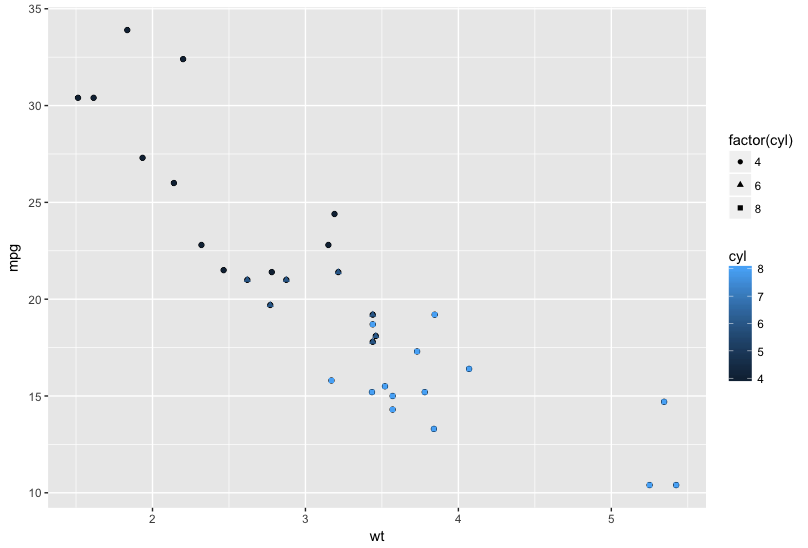
\includegraphics[scale=0.45]{ilu/bg40.png}\end{center}\end{figure}
\begin{lstlisting}[language=html]
# Change shape, color, size manually
# Change the point sizes manually
> b + geom_point(aes(color = cyl, shape=factor(cyl), size = factor(cyl))) + scale_size_manual(values = c(2,3,4))
\end{lstlisting}
\begin{figure}[H]\begin{center}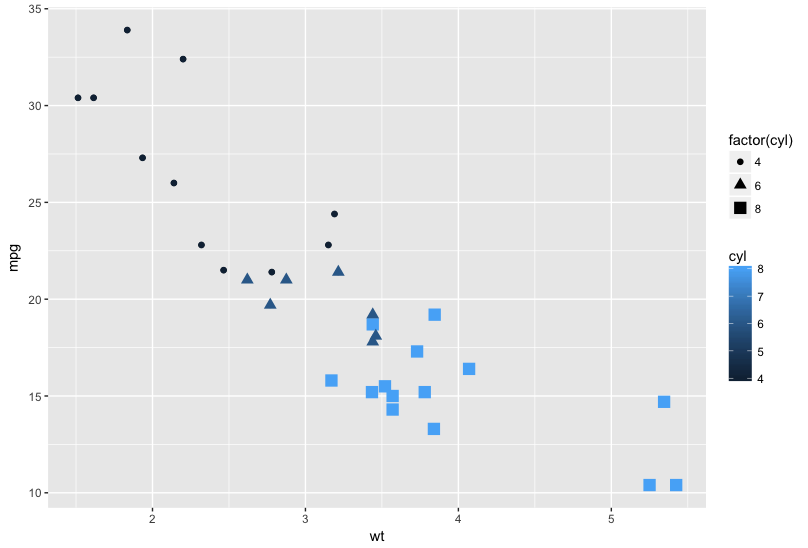
\includegraphics[scale=0.45]{ilu/bg41.png}\end{center}\end{figure}
\begin{lstlisting}[language=html]
# Change the point shapes and colors manually
> b + geom_point(aes(color = cyl, shape = cyl)) + scale_shape_manual(values = c(3,16,17)) + scale_color_manual(values = c('#999999','#E69F00', '#56B4E9'))
Erreur : Continuous value supplied to discrete scale
\end{lstlisting}
\begin{figure}[H]\begin{center}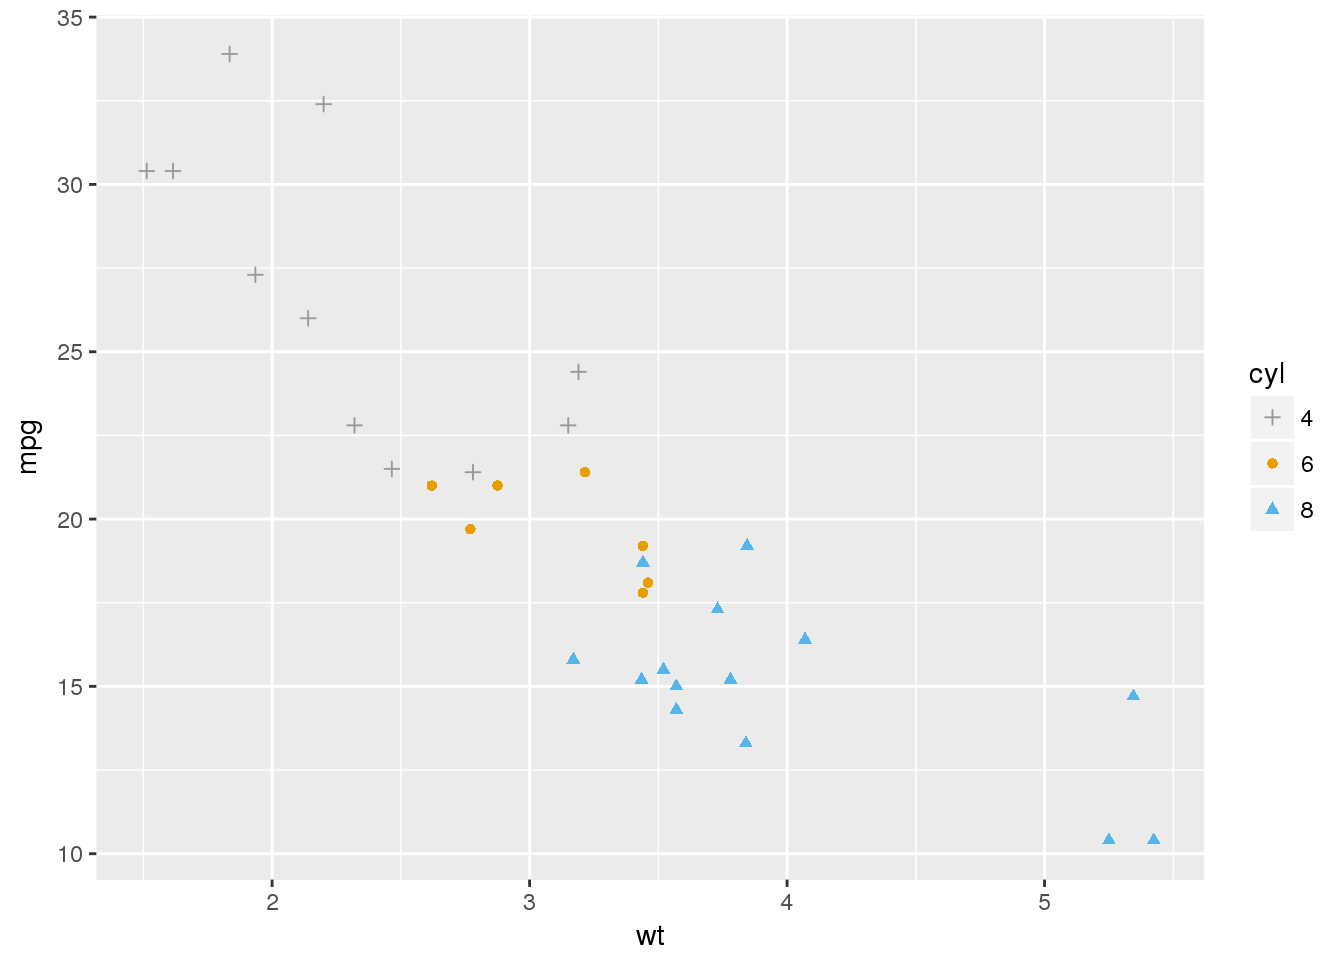
\includegraphics[scale=0.45]{ilu/bg42.png}\end{center}\end{figure}
\begin{lstlisting}[language=html]
# Use brewer color palettes
> b + geom_point(aes(color = cyl, shape = factor(cyl))) + scale_color_brewer(palette = "Dark2") + theme_minimal()
Erreur : Continuous value supplied to discrete scale
\end{lstlisting}
\begin{figure}[H]\begin{center}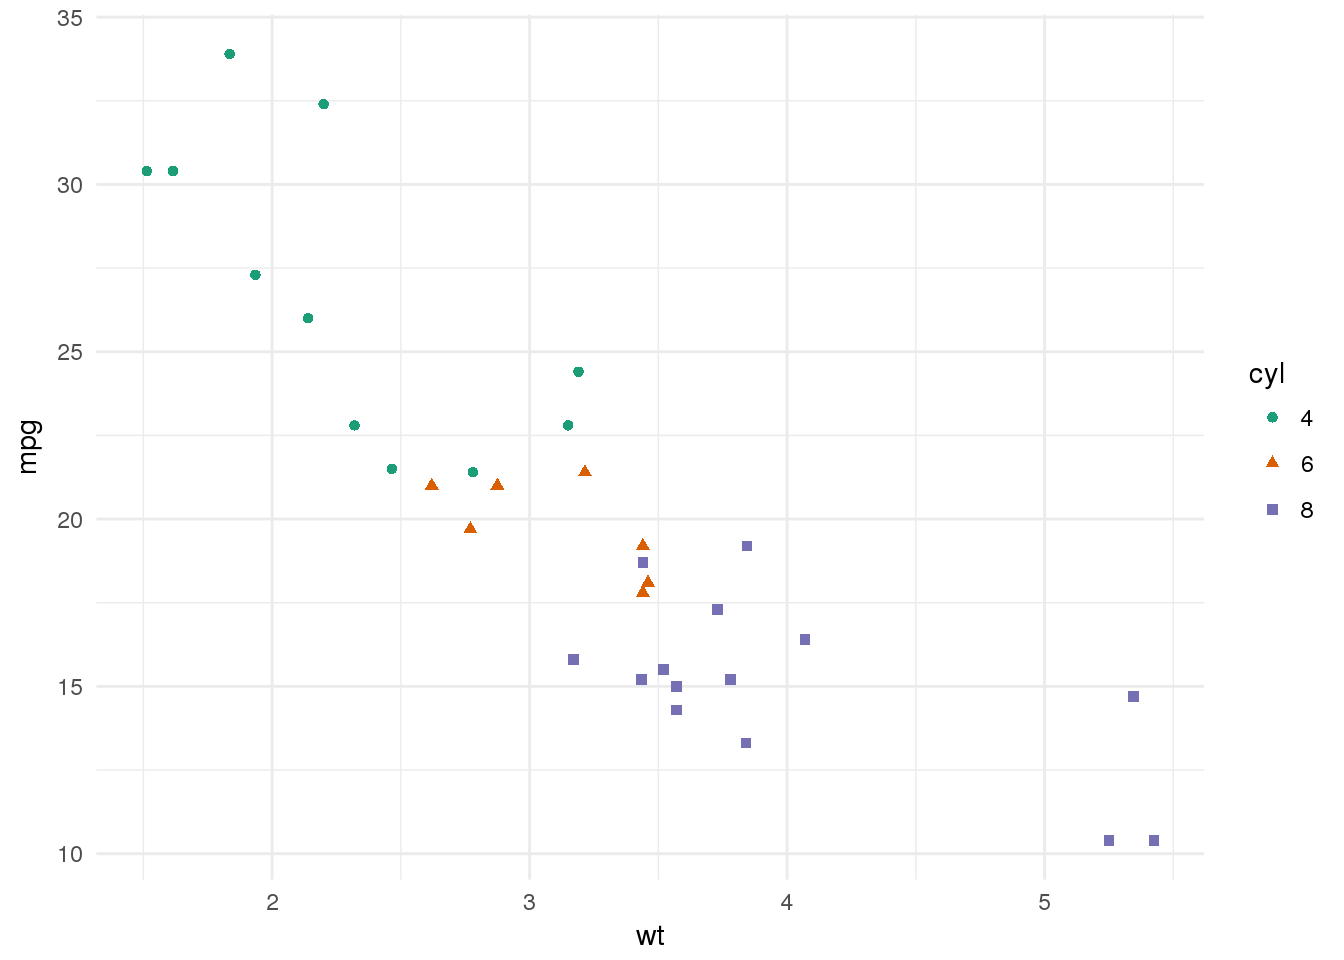
\includegraphics[scale=0.45]{ilu/bg43.png}\end{center}\end{figure}
\begin{lstlisting}[language=html]
# Use grey scale
> b + geom_point(aes(color = cyl, shape = factor(cyl))) + scale_color_grey() + theme_minimal()
Erreur : Continuous value supplied to discrete scale
\end{lstlisting}
\begin{figure}[H]\begin{center}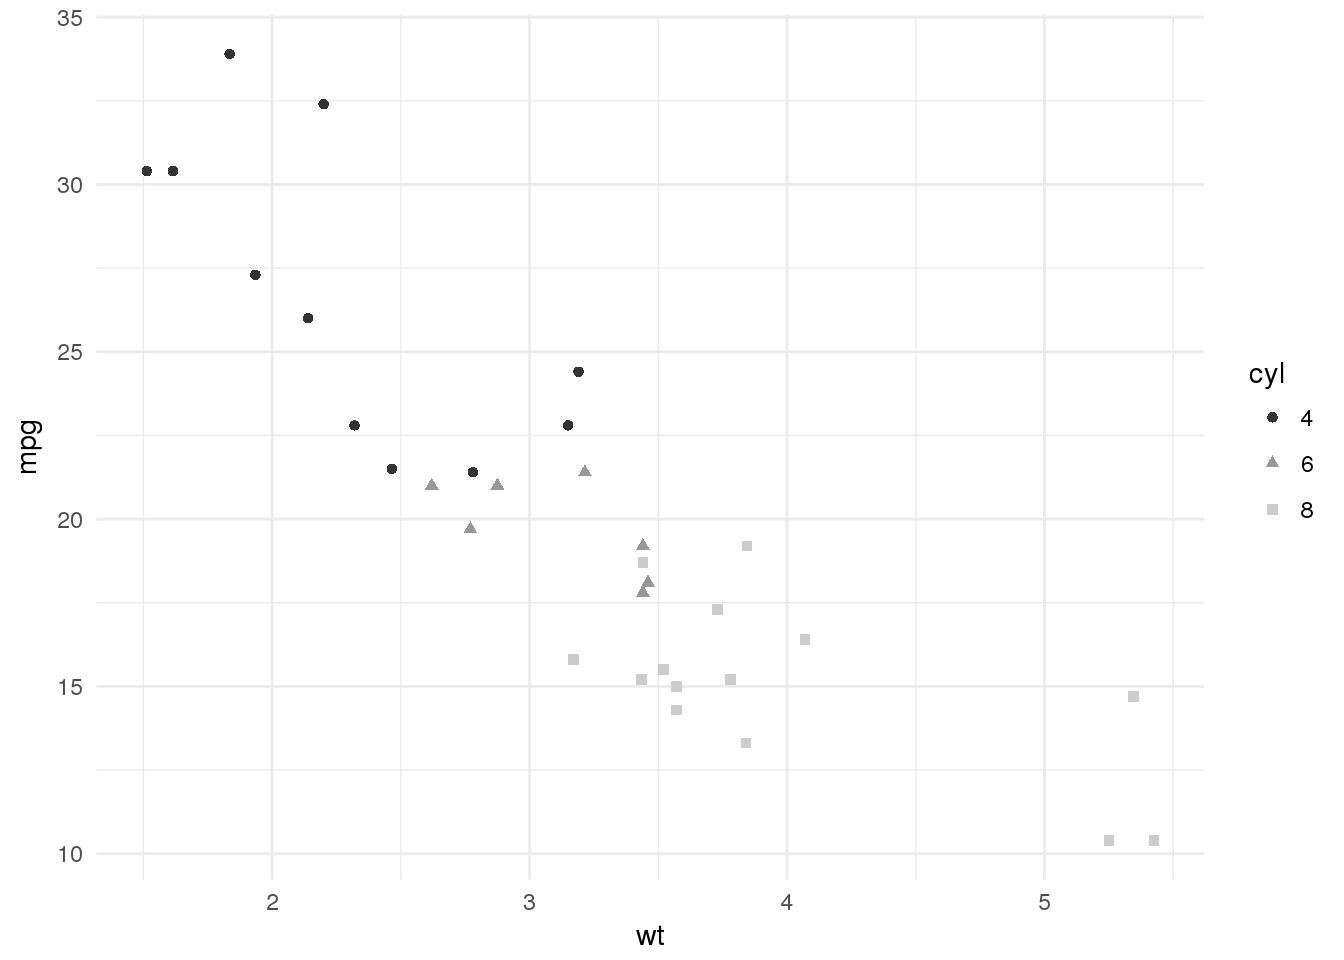
\includegraphics[scale=0.45]{ilu/bg44.png}\end{center}\end{figure}

\textbf{Add regression line or smoothed conditional mean}
\begin{lstlisting}[language=html]
#geom_smooth(), geom_abline()
#alpha, color, fill, shape, linetype, size
#geom_smooth(method = "auto")
#method:loess->local regression, lm-> linear regression

# Add regression line
> b + geom_point() + geom_smooth(method = lm)
\end{lstlisting}
\begin{figure}[H]\begin{center}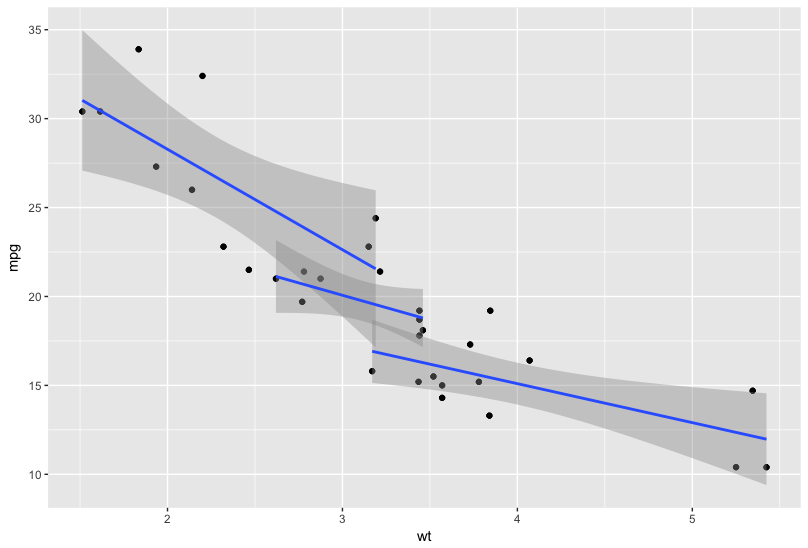
\includegraphics[scale=0.45]{ilu/bg45.png}\end{center}\end{figure}
\begin{lstlisting}[language=html]
# Point + regression line
# Remove the confidence interval
> b + geom_point() + geom_smooth(method = lm, se = FALSE)
\end{lstlisting}
\begin{figure}[H]\begin{center}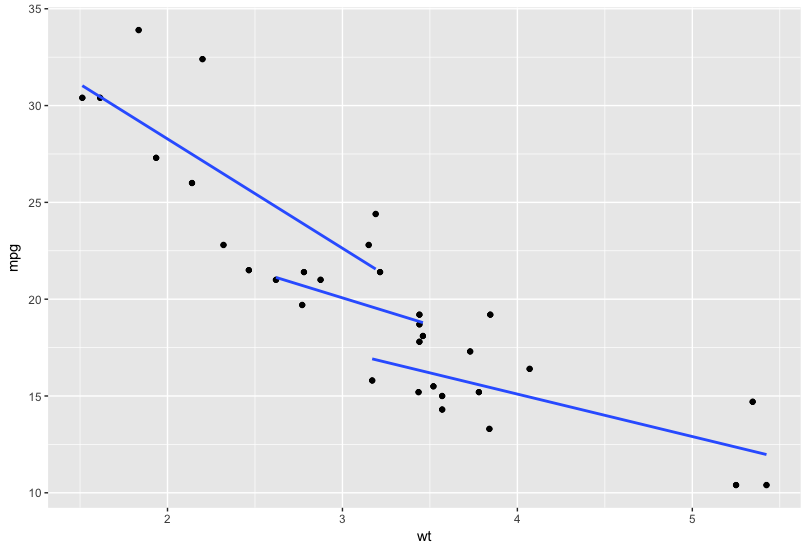
\includegraphics[scale=0.45]{ilu/bg46.png}\end{center}\end{figure}
\begin{lstlisting}[language=html]
# loess method, local regression fitting
> b + geom_point() + geom_smooth()
\end{lstlisting}
\begin{figure}[H]\begin{center}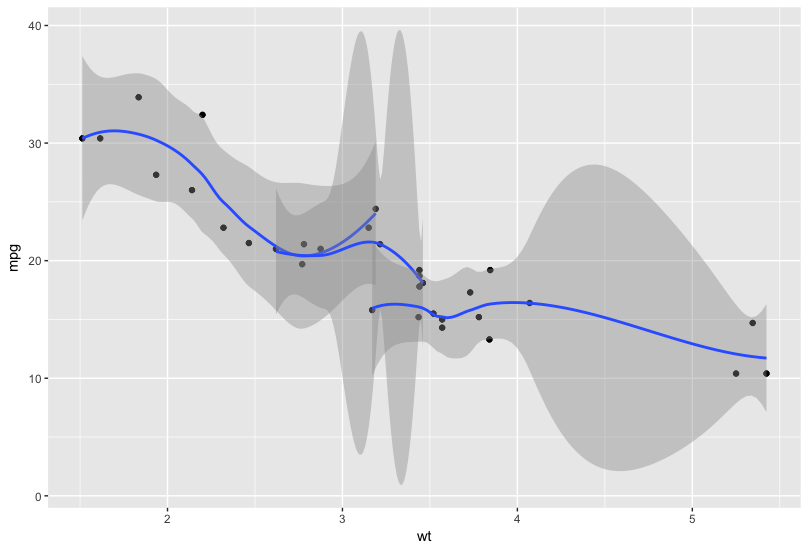
\includegraphics[scale=0.45]{ilu/bg47.png}\end{center}\end{figure}
\begin{lstlisting}[language=html]
# Change the color and shape by groups 
> b + geom_point(aes(color = cyl, shape = factor(cyl))) + geom_smooth(aes(color = cyl, fill = cyl), method = lm)
\end{lstlisting}
\begin{figure}[H]\begin{center}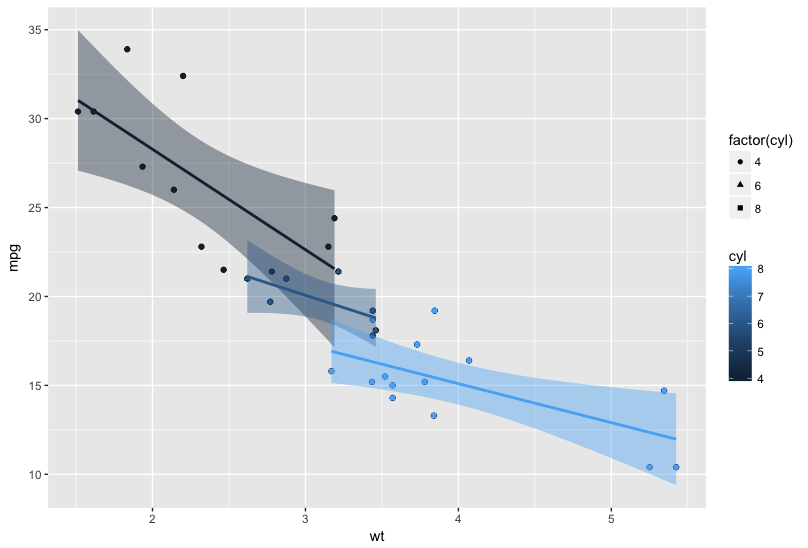
\includegraphics[scale=0.45]{ilu/bg48.png}\end{center}\end{figure}
\begin{lstlisting}[language=html]
# Remove confidence intervals
# Extend the regression lines: fullrage
> b + geom_point(aes(color = cyl, shape = factor(cyl))) + geom_smooth(aes(color = cyl), method = lm, se = FALSE, fullrange = TRUE)
\end{lstlisting}
\begin{figure}[H]\begin{center}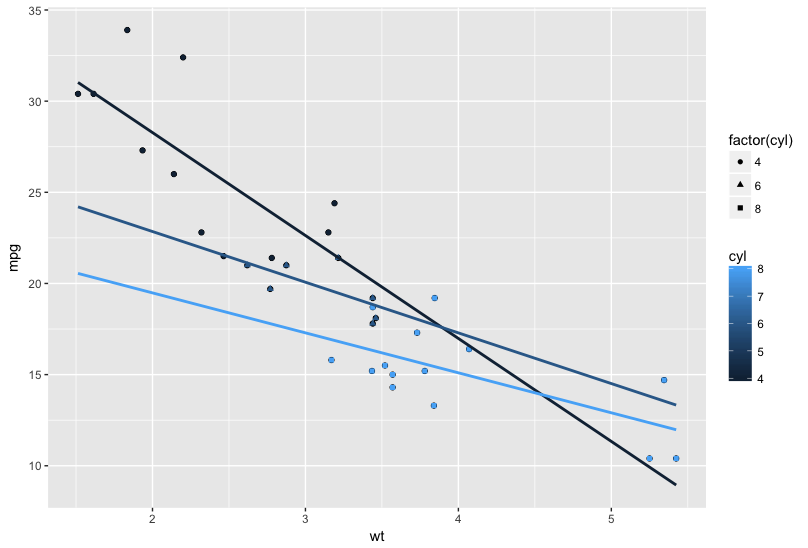
\includegraphics[scale=0.45]{ilu/bg49.png}\end{center}\end{figure}
\begin{lstlisting}[language=html]
# Add marginal rugs to a scatter plot
#geom_rug(sides = "bl")
# sides: a string, "trbl", top, right, bottom, left.
# Add marginal rugs
> b + geom_point() + geom_rug()
\end{lstlisting}
\begin{figure}[H]\begin{center}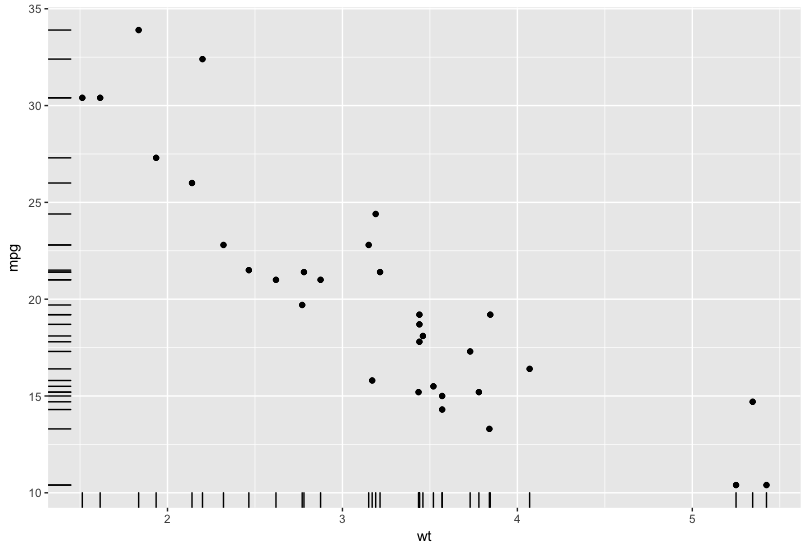
\includegraphics[scale=0.45]{ilu/bg50.png}\end{center}\end{figure}
\begin{lstlisting}[language=html]
# Change the color by group
> b + geom_point(aes(color = cyl)) + geom_rug(aes(color = cyl))
\end{lstlisting}
\begin{figure}[H]\begin{center}\includegraphics[scale=0.45]{ilu/bg51.png}\end{center}\end{figure}
\begin{lstlisting}[language=html]
# Add marginal rugs using faithful data
> data(faithful)
> faithful <- as_data_frame(faithful)
> faithful
# A tibble: 272 x 2
   eruptions waiting
 *     <dbl>   <dbl>
 1     3.600      79
 2     1.800      54
 3     3.333      74
 4     2.283      62
 5     4.533      85
 6     2.883      55
 7     4.700      88
 8     3.600      85
 9     1.950      51
10     4.350      85
# ... with 262 more rows
\end{lstlisting}
\textcolor{white}{.}\newline
\begin{lstlisting}[language=html]
> ggplot(faithful, aes(x = eruptions, y = waiting)) + geom_point() + geom_rug()
\end{lstlisting}
\begin{figure}[H]\begin{center}\includegraphics[scale=0.45]{ilu/bg52.png}\end{center}\end{figure}
\begin{lstlisting}[language=html]
# Jitter points to reduce overplotting
# geom_jitter(), position_jitter()
#alpha, color, fill, shape, size

# Use mpg data
> p <- ggplot(mpg, aes(displ, hwy))

# Default sactter plot
> p + geom_point()
\end{lstlisting}
\begin{figure}[H]\begin{center}\includegraphics[scale=0.45]{ilu/bg53.png}\end{center}\end{figure}
\begin{lstlisting}[language=html]
# Use jitter to reduce overplotting
> p + geom_jitter(position = position_jitter(width = 0.5, height = 0.5))
\end{lstlisting}
\begin{figure}[H]\begin{center}\includegraphics[scale=0.45]{ilu/bg54.png}\end{center}\end{figure}
\begin{lstlisting}[language=html]
> select(mpg, displ, hwy) %>% arrange(-hwy) %>% filter(displ == 1.9)
# A tibble: 3 x 2
  displ   hwy
  <dbl> <int>
1   1.9    44
2   1.9    44
3   1.9    41
\end{lstlisting}
\textcolor{white}{.}\newline
\begin{lstlisting}[language=html]
##
#Text annotation
#geom_text()
#label, alpha, angle, color, family, fontface, hjust, lineheight, size, vjust

> b + geom_text(aes(label = rownames(mtcars)), size = 3)
\end{lstlisting}
\begin{figure}[H]\begin{center}\includegraphics[scale=0.45]{ilu/bg55.png}\end{center}\end{figure}

\subsection{Continuous bivariate distribution}
\begin{itemize}
  \item geom\_bin2d()
  \item geom\_hex()
  \item geom\_density\_2d()
\end{itemize}

\begin{lstlisting}[language=html]
> data("diamonds")
> c <- ggplot(diamonds, aes(carat, price))
# Add heatmap of 2d bin counts
# geom_bin2d produce a scatter plot with rectangular bins.
# stat_bin_2d(), stat_summary_2d()
# max, xmin, ymax, ymin, alpha, color, fill, linetype, size
> c + geom_bin2d()
\end{lstlisting}
\begin{figure}[H]\begin{center}\includegraphics[scale=0.45]{ilu/bg56.png}\end{center}\end{figure}
\begin{lstlisting}[language=html]
# Change the number of bins
> c + geom_bin2d(bins = 15)
\end{lstlisting}
\begin{figure}[H]\begin{center}\includegraphics[scale=0.45]{ilu/bg57.png}\end{center}\end{figure}
\begin{lstlisting}[language=html]
# Specify the width of bins
> c + geom_bin2d(binwidth = c(1,1000))
\end{lstlisting}
\begin{figure}[H]\begin{center}\includegraphics[scale=0.45]{ilu/bg58.png}\end{center}\end{figure}
\begin{lstlisting}[language=html]
> c + stat_bin_2d()
\end{lstlisting}
\begin{figure}[H]\begin{center}\includegraphics[scale=0.45]{ilu/bg59.png}\end{center}\end{figure}
\begin{lstlisting}[language=html]
> c + stat_summary_2d(aes(z = depth))
\end{lstlisting}
\begin{figure}[H]\begin{center}\includegraphics[scale=0.45]{ilu/bg60.png}\end{center}\end{figure}
\begin{lstlisting}[language=html]
# Add hexagon bining
#geom_hex()
# stat_bin_hex(), stat_summary_hex()
# alpha, color, fill, size
> install.packages("hexbin")
> library(hexbin)

> c + geom_hex()
\end{lstlisting}
\begin{figure}[H]\begin{center}\includegraphics[scale=0.45]{ilu/bg61.png}\end{center}\end{figure}
\begin{lstlisting}[language=html]
# Change the number of bins
> c + geom_hex(bins = 10)
\end{lstlisting}
\begin{figure}[H]\begin{center}\includegraphics[scale=0.45]{ilu/bg62.png}\end{center}\end{figure}
\begin{lstlisting}[language=html]
> c + stat_bin_hex()
\end{lstlisting}
\begin{figure}[H]\begin{center}\includegraphics[scale=0.45]{ilu/bg63.png}\end{center}\end{figure}
\begin{lstlisting}[language=html]
> c + stat_summary_hex(aes(z = depth))
\end{lstlisting}
\begin{figure}[H]\begin{center}\includegraphics[scale=0.45]{ilu/bg64.png}\end{center}\end{figure}
\begin{lstlisting}[language=html]
# 2D density estimation
# geom_density_2d()
# stat_density_2d()
# alpha, color, linetype, size

# Scatter plot
> sp <- ggplot(faithful, aes(x = eruptions, y = waiting))
> select(faithful, eruptions, waiting)
# A tibble: 272 x 2
   eruptions waiting
 *     <dbl>   <dbl>
 1     3.600      79
 2     1.800      54
 3     3.333      74
 4     2.283      62
 5     4.533      85
 6     2.883      55
 7     4.700      88
 8     3.600      85
 9     1.950      51
10     4.350      85
# ... with 262 more rows
\end{lstlisting}
\begin{lstlisting}[language=html]
# Default plot
> sp + geom_density_2d(color = "#E7B800")
\end{lstlisting}
\begin{figure}[H]\begin{center}\includegraphics[scale=0.45]{ilu/bg65.png}\end{center}\end{figure}
\begin{lstlisting}[language=html]
# Add points
> sp + geom_point(color = "#00AFBB") + geom_density_2d(color = "#E7B800")
\end{lstlisting}
\begin{figure}[H]\begin{center}\includegraphics[scale=0.45]{ilu/bg66.png}\end{center}\end{figure}
\begin{lstlisting}[language=html]
# Use stat_density_2d with geom = "polygon"
sp + geom_point() + stat_density_2d(aes(fill = ..level..), geom = "polygon")
\end{lstlisting}
\begin{figure}[H]\begin{center}\includegraphics[scale=0.45]{ilu/bg67.png}\end{center}\end{figure}
\begin{lstlisting}[language=html]
# Change the gradient color
> sp + geom_point() + stat_density_2d(aes(fill = ..level..), geom = "polygon") + scale_fill_gradient(low = "#00AFBB", high = "#FC3E07")
\end{lstlisting}
\begin{figure}[H]\begin{center}\includegraphics[scale=0.45]{ilu/bg68.png}\end{center}\end{figure}
\begin{lstlisting}[language=html]
# Gradient
\end{lstlisting}
\subsection{Two variables: Discrete X, Discrete Y}

\textbf{geom\_jitter\newline
alpha, color, fill, shape, size}
\begin{lstlisting}[language=html]
> ggplot(diamonds, aes(cut, color)) + geom_jitter(aes(color = cut), size = 0.5)
\end{lstlisting}
\begin{figure}[H]\begin{center}\includegraphics[scale=0.45]{ilu/bg69.png}\end{center}\end{figure}
\begin{lstlisting}[language=html]
> select(diamonds, cut, color)
# A tibble: 53,940 x 2
         cut color
       <ord> <ord>
 1     Ideal     E
 2   Premium     E
 3      Good     E
 4   Premium     I
 5      Good     J
 6 Very Good     J
 7 Very Good     I
 8 Very Good     H
 9      Fair     E
10 Very Good     H
# ... with 53,930 more rows
\end{lstlisting}

\section{Plot Two Variables - X \& Y: Discrete X and Continuous Y}
\begin{itemize}
  \item geom\_boxplot()
  \item geom\_violin()
  \item geom\_dotplot()
  \item geom\_jitter()
  \item geom\_line()
  \item geom\_bar()

\end{itemize}

\begin{lstlisting}[language=html]
> data("ToothGrowth")
> ToothGrowth$dose <- as.factor(ToothGrowth$dose)
> ToothGrowth <- as_data_frame(ToothGrowth)
> ToothGrowth
# A tibble: 60 x 3
     len   supp   dose
   <dbl> <fctr> <fctr>
 1   4.2     VC    0.5
 2  11.5     VC    0.5
 3   7.3     VC    0.5
 4   5.8     VC    0.5
 5   6.4     VC    0.5
 6  10.0     VC    0.5
 7  11.2     VC    0.5
 8  11.2     VC    0.5
 9   5.2     VC    0.5
10   7.0     VC    0.5
# ... with 50 more rows
\end{lstlisting}
\textcolor{white}{.}\newline
\begin{lstlisting}[language=html]
## Chargement de e
e <- ggplot(ToothGrowth, aes(x = dose, y = len))
\end{lstlisting}
\subsection{Box Plots}

\textbf{alpha, color, linetype, shape, size, fill}\newline
\begin{lstlisting}[language=html]
> geom_boxplot(outlier.colour = "black", outlier.shape = 16, outlier.size = 2, notch = FALSE)
\end{lstlisting}
\textcolor{white}{.}\newline
\begin{lstlisting}[language=html]
# Basic box plot
> e + geom_boxplot()
\end{lstlisting}
\begin{figure}[H]\begin{center}\includegraphics[scale=0.45]{ilu/bg70.png}\end{center}\end{figure}
\begin{lstlisting}[language=html]
# Rotate the box plot
> e + geom_boxplot() + coord_flip()
\end{lstlisting}
\begin{figure}[H]\begin{center}\includegraphics[scale=0.45]{ilu/bg71.png}\end{center}\end{figure}
\begin{lstlisting}[language=html]
# Notched box plot
> e + geom_boxplot(notch = TRUE)
\end{lstlisting}
\begin{figure}[H]\begin{center}\includegraphics[scale=0.45]{ilu/bg72.png}\end{center}\end{figure}
\begin{lstlisting}[language=html]
# Box plot with mean points
> e + geom_boxplot() + stat_summary(fun.y = mean, geom = "point", shape = 18, size = 4, color = "blue")
\end{lstlisting}
\begin{figure}[H]\begin{center}\includegraphics[scale=0.45]{ilu/bg73.png}\end{center}\end{figure}
\begin{lstlisting}[language=html]
# chose which item to display
> e + geom_boxplot() + scale_x_discrete(limits = c("0.5", "2"))
\end{lstlisting}
\begin{figure}[H]\begin{center}\includegraphics[scale=0.45]{ilu/bg74.png}\end{center}\end{figure}
\begin{lstlisting}[language=html]
# change default order of items
> e + geom_boxplot() + scale_x_discrete(limits = c("2", "0.5", "1"))
\end{lstlisting}
\begin{figure}[H]\begin{center}\includegraphics[scale=0.45]{ilu/bg75.png}\end{center}\end{figure}
\begin{lstlisting}[language=html]
> e + stat_boxplot(coeff = 1.5)
## Warning: Ignoring unknown parameters: coeff
\end{lstlisting}
\begin{figure}[H]\begin{center}\includegraphics[scale=0.45]{ilu/bg76.png}\end{center}\end{figure}

\textbf{Change the color by group :} box plot outline and fill colors can be automatically controlled by the levels of the grouping variable \textit{dose}
\begin{lstlisting}[language=html]
# Use single color
> e + geom_boxplot(color = "black", fill = "steelblue")
\end{lstlisting}
\begin{figure}[H]\begin{center}\includegraphics[scale=0.45]{ilu/bg77.png}\end{center}\end{figure}
\begin{lstlisting}[language=html]
# Change outline colors by dose (groups)
> e + geom_boxplot(aes(color = dose))
\end{lstlisting}
\begin{figure}[H]\begin{center}\includegraphics[scale=0.45]{ilu/bg78.png}\end{center}\end{figure}
\begin{lstlisting}[language=html]
# Change the fill color by dose (groups)
> e + geom_boxplot(aes(fill = dose))
\end{lstlisting}
\begin{figure}[H]\begin{center}\includegraphics[scale=0.45]{ilu/bg79.png}\end{center}\end{figure}
\begin{lstlisting}[language=html]
# Change munually outline colors:
# Use custom color palettes
> e2 <- e + geom_boxplot(aes(color = dose)) + theme_minimal()
> e2 + scale_color_manual(values = c("#999999", "#E69F00", "#56B4E9"))
\end{lstlisting}
\begin{figure}[H]\begin{center}\includegraphics[scale=0.45]{ilu/bg80.png}\end{center}\end{figure}
\begin{lstlisting}[language=html]
# Use brewer color palettes
> e2 + scale_color_brewer(palette  = "Dark2")
\end{lstlisting}
\begin{figure}[H]\begin{center}\includegraphics[scale=0.45]{ilu/bg81.png}\end{center}\end{figure}
\begin{lstlisting}[language=html]
# Use grey scale
> e2 + scale_color_grey()
\end{lstlisting}
\begin{figure}[H]\begin{center}\includegraphics[scale=0.45]{ilu/bg82.png}\end{center}\end{figure}
\begin{lstlisting}[language=html]
## Change manually by fill color
# Use the custom color palettes
> e3 <- e + geom_boxplot(aes(fill = dose)) + theme_minimal()
> e3 + scale_fill_manual(values = c("#999999", "#E69F00", "#56B4E9"))
\end{lstlisting}
\begin{figure}[H]\begin{center}\includegraphics[scale=0.45]{ilu/bg83.png}\end{center}\end{figure}
\begin{lstlisting}[language=html]
# Use brewer color palettes
> e3 + scale_fill_brewer(palette = "Dark2")
\end{lstlisting}
\begin{figure}[H]\begin{center}\includegraphics[scale=0.45]{ilu/bg84.png}\end{center}\end{figure}
\begin{lstlisting}[language=html]
# Use grey color
> e3 + scale_fill_grey()
\end{lstlisting}
\begin{figure}[H]\begin{center}\includegraphics[scale=0.45]{ilu/bg85.png}\end{center}\end{figure}

\textbf{Boxplot with multiple groups : } The grouping variable \textit{dose} and \textit{supp} are used :
\begin{lstlisting}[language=html]
# Change box plot colors by groups
e + geom_boxplot(aes(fill = supp))
\end{lstlisting}
\begin{figure}[H]\begin{center}\includegraphics[scale=0.45]{ilu/bg86.png}\end{center}\end{figure}
\begin{lstlisting}[language=html]
# Change the position
e + geom_boxplot(aes(fill = supp), position = position_dodge(1.1))
\end{lstlisting}
\begin{figure}[H]\begin{center}\includegraphics[scale=0.45]{ilu/bg87.png}\end{center}\end{figure}
\begin{lstlisting}[language=html]
# Change the fill color
e + geom_boxplot(aes(fill = supp), position = position_dodge(1.1)) + scale_fill_brewer("BrBG")
\end{lstlisting}
\begin{figure}[H]\begin{center}\includegraphics[scale=0.45]{ilu/bg88.png}\end{center}\end{figure}

\subsection{Violin Plots}
Violin plots is similar to boxplot, except that they also show the kernel probability density of the data at different values. Tipically, violin plots will include a marker for the median of the data and a box indicating the interquartile range, as in standard boxplots.\newline
\\
\textbf{alpha, color, fill, linetype, size, and fill}
\begin{lstlisting}[language=html]
# Basic plot
> e + geom_violin()
\end{lstlisting}
\begin{figure}[H]\begin{center}\includegraphics[scale=0.45]{ilu/bg89.png}\end{center}\end{figure}
\begin{lstlisting}[language=html]
# Rotate the violin plot
> e + geom_violin() + coord_flip()
\end{lstlisting}
\begin{figure}[H]\begin{center}\includegraphics[scale=0.45]{ilu/bg90.png}\end{center}\end{figure}
\begin{lstlisting}[language=html]
# Set trim argument to FALSE
> e + geom_violin(trim = FALSE, fill = "steelblue")
\end{lstlisting}
\begin{figure}[H]\begin{center}\includegraphics[scale=0.45]{ilu/bg91.png}\end{center}\end{figure}

\textbf{Add summary statistics : } Funtion stat\_summary() can be used to add mean/median points and more on a violin plot
\begin{lstlisting}[language=html]
# Add mean and median points: use fun.y = mean or fun.y = median
e + geom_violin(trim = FALSE) + stat_summary(fun.y = mean, geom = "point", shape = 23, size = 2, color = "blue")
\end{lstlisting}

\begin{figure}[H]\begin{center}\includegraphics[scale=0.45]{ilu/bg92.png}\end{center}\end{figure}
\begin{lstlisting}[language=html]
# Add mean points +/- SD
# Use geom = "pointrange" or geom = "crossbar"
> library("Hmisc") ## stat_summary
> e + geom_violin(trim = FALSE) + stat_summary(fun.data = "mean_sdl", fun.args = list(mult = 1), geom = "pointrange", color = "red")
\end{lstlisting}
\begin{figure}[H]\begin{center}\includegraphics[scale=0.45]{ilu/bg93.png}\end{center}\end{figure}


The function \textit{mean\_sdl} is used for adding mean and standard deviation. It computes the mean plus or minus a constant times the standard deviation. The constant is specified using the argument\textit{mult} (\textit{mult} = 1). Default \textit{mult = 2}.\newline
The mean $\pm$ SD can be added as crossbar or a pointrange. 
\begin{lstlisting}[language=html]
# Combine with box plot to add median and quartiles
> e + geom_violin(trim = FALSE) + geom_boxplot(width = 0.2)
\end{lstlisting}
\begin{figure}[H]\begin{center}\includegraphics[scale=0.45]{ilu/bg94.png}\end{center}\end{figure}

\textbf{Change colors by groups : } The color and fill can be automatically controlled by the levels  of the grouping variable dose. 
\begin{lstlisting}[language=html]
# Change the outline colors by dose (groups)
> e + geom_violin(aes(color = dose), trim = FALSE)
\end{lstlisting}
\begin{figure}[H]\begin{center}\includegraphics[scale=0.45]{ilu/bg95.png}\end{center}\end{figure}
\begin{lstlisting}[language=html]
# Change the fill color by dose
> e  + geom_violin(aes(fill = dose), trim = FALSE)
\end{lstlisting}
\begin{figure}[H]\begin{center}\includegraphics[scale=0.45]{ilu/bg96.png}\end{center}\end{figure}
\begin{lstlisting}[language=html]
# Change outline and fill color manually.
> e2 <- e + geom_violin(aes(color = dose), trim = FALSE) + theme_minimal()
> e2 + scale_color_brewer(palette = "Dark2")
\end{lstlisting}
\begin{figure}[H]\begin{center}\includegraphics[scale=0.45]{ilu/bg97.png}\end{center}\end{figure}
\begin{lstlisting}[language=html]
# Change manually fill colors
> e3 <- e + geom_violin(aes(fill = dose), trim = FALSE) + theme_minimal()
> e3 + scale_fill_brewer(palette = "Dark2")
\end{lstlisting}
\begin{figure}[H]\begin{center}\includegraphics[scale=0.45]{ilu/bg98.png}\end{center}\end{figure}

\begin{lstlisting}[language=html]
## Violin plot with multiple groups
# Change the color by groups
> e + geom_violin(aes(fill = supp), trim = FALSE)
\end{lstlisting}
\begin{figure}[H]\begin{center}\includegraphics[scale=0.45]{ilu/bg99.png}\end{center}\end{figure}
\begin{lstlisting}[language=html]
# Change fill colors
> e + geom_violin(aes(fill = supp), trim = FALSE) + scale_fill_brewer(palette = "Dark2")
\end{lstlisting}

\begin{figure}[H]\begin{center}\includegraphics[scale=0.45]{ilu/bg100.png}\end{center}\end{figure}

\subsection{Dot plots}
geom\_dotplot(), stat\_summary() (package : "Hmisc")\newline
\\
\textbf{alpha, color, dotsize and fill}
\begin{lstlisting}[language=html]
#Basic dot plot
> e + geom_dotplot(binaxis ="y", stackdir = "center")
\end{lstlisting}
\begin{figure}[H]\begin{center}\includegraphics[scale=0.45]{ilu/bg101.png}\end{center}\end{figure}
\begin{lstlisting}[language=html]
# Change dotsize and stack ratio
> e + geom_dotplot(binaxis = "y", stackdir = "center", stackratio = 1.5, dotsize = 1.1)
\end{lstlisting}
\begin{figure}[H]\begin{center}\includegraphics[scale=0.45]{ilu/bg102.png}\end{center}\end{figure}

\textit{stat\_summary()} can be used to add mean/median points and more on a violin plot.
\begin{lstlisting}[language=html]
# Add mean and median points: use fun.y = mean or fun.y = median
> e + geom_dotplot(binaxis = "y", stackdir = "center") + stat_summary(fun.y = mean, geom = "point", shape = 18, size = 3, color = "red")
\end{lstlisting}
\begin{figure}[H]\begin{center}\includegraphics[scale=0.45]{ilu/bg103.png}\end{center}\end{figure}
\begin{lstlisting}[language=html]
# Add mean points with +/- SD
# Use geom = "pointrange" or geom = "crossbar"
> e + geom_dotplot(binaxis = "y", stackdir = "center") + stat_summary(fun.data = "mean_sdl", fun.args = list(mult = 1), geom = "pointrange", color = "red")
\end{lstlisting}
\begin{figure}[H]\begin{center}\includegraphics[scale=0.45]{ilu/bg104.png}\end{center}\end{figure}

Combine with box plot and dot plot:
\begin{lstlisting}[language=html]
# Combine with boxplot
> e + geom_boxplot() + geom_dotplot(binaxis = "y", stackdir ="center")
\end{lstlisting}
\begin{figure}[H]\begin{center}\includegraphics[scale=0.45]{ilu/bg105.png}\end{center}\end{figure}
%%%%%%%%%%%%%%%%%%%%%%%%%%%%%%%%%%%%%%%%%%%%%%%%%%%%%%%%%%%%%%%%%%%%%%%%%%%%%%
\begin{lstlisting}[language=html]
# Combine with violin plot
> e + geom_violin(trim = FALSE) + geom_dotplot(binaxis = "y", stackdir ="center")
\end{lstlisting}
\begin{figure}[H]\begin{center}\includegraphics[scale=0.45]{ilu/bg106.png}\end{center}\end{figure}
\begin{lstlisting}[language=html]
# Dotplot + violin plot + stat summary
> e + geom_violin(trim = FALSE) + geom_dotplot(binaxis = "y", stackdir ="center") + stat_summary(fun.data = "mean_sdl", fun.args = list(mult = 1), geom = "pointrange", color = "red", shape = 11)
\end{lstlisting}
\begin{figure}[H]\begin{center}\includegraphics[scale=0.45]{ilu/bg107.png}\end{center}\end{figure}

Use scale to change the outlien and fill color automatically controlled byt the levels of the grouping variable dose : 
\begin{itemize}
  \item scale\_color\_munual(), scale\_color\_brewer(), scale\_color\_grey()
  \item scale\_fill\_munual(), sclae\_fill\_brewer(), scale\_fill\_grey()
\end{itemize}
 
\begin{figure}[H]\begin{center}\includegraphics[scale=0.45]{ilu/bg108.png}\end{center}\end{figure} 

Dotplot with multiple groups, just like boxplot and violin plot

\subsection{Stripcharts}
Stripecharts are also known as one dimensional scatter plots. These plots are suitable compared to box plot when sample sizes are small.\newline
\textit{geom\_jitter(), stat\_summary()}.\newline
\\
\textbf{alpha, color, size and fill}
\begin{lstlisting}[language=html]
> e <- ggplot(ToothGrowth, aes(x = dose, y = len))
> e + geom_jitter()
\end{lstlisting}
\begin{figure}[H]\begin{center}\includegraphics[scale=0.45]{ilu/bg109.png}\end{center}\end{figure} 
\begin{lstlisting}[language=html]
# Change the position
# 0.2 is the degree of jitter in x direction
> e + geom_jitter(position = position_jitter(0.2))
\end{lstlisting}
\begin{figure}[H]\begin{center}\includegraphics[scale=0.45]{ilu/bg110.png}\end{center}\end{figure} 
\begin{lstlisting}[language=html]
# Change point shapes and size
> e  + geom_boxplot()+ geom_jitter(position = position_jitter(0.2), shape = 11, size = 1.2)
\end{lstlisting}
\begin{figure}[H]\begin{center}\includegraphics[scale=0.45]{ilu/bg111.png}\end{center}\end{figure} 
\begin{lstlisting}[language=html]
# Add summary statistics
# Add mean or median point
> e + geom_jitter(position = position_jitter(0.2)) + stat_summary(fun.y = mean, geom = "point", shape = 18, size = 3, color = "red")
\end{lstlisting}
\begin{figure}[H]\begin{center}\includegraphics[scale=0.45]{ilu/bg112.png}\end{center}\end{figure} 
\begin{lstlisting}[language=html]
# use geom = "pointrange"
> e + geom_jitter(position = position_jitter(0.2)) + stat_summary(fun.data = "mean_sdl", fun.args = list(mult = 1), shape = 18, color = "red")
\end{lstlisting}
\begin{figure}[H]\begin{center}\includegraphics[scale=0.45]{ilu/bg113.png}\end{center}\end{figure}
\begin{lstlisting}[language=html]
# Combine with boxplot and violin plot
> e + geom_violin(trim = FALSE) + geom_jitter(position = position_jitter(0.1)) + stat_summary(fun.data = "mean_sdl", fun.args = list(mult = 1), shape = 18, color = "red")
\end{lstlisting}
\begin{figure}[H]\begin{center}\includegraphics[scale=0.45]{ilu/bg114.png}\end{center}\end{figure}
\begin{lstlisting}[language=html]
# Change point shape by group
> e + geom_jitter(aes(shape = dose), position = position_jitter(0.2)) + scale_shape_manual(values = c(1,17,19))
\end{lstlisting}
\begin{figure}[H]\begin{center}\includegraphics[scale=0.45]{ilu/bg115.png}\end{center}\end{figure}
\begin{lstlisting}[language=html]
# Change color by groups
> e + geom_jitter(aes(color = dose, shape = dose), position = position_jitter(0.2)) + theme_minimal()
\end{lstlisting}
\begin{figure}[H]\begin{center}\includegraphics[scale=0.45]{ilu/bg116.png}\end{center}\end{figure}

\textbf{Change the outlien and fill color by scale : } Stripchar with multiple groups.
\begin{lstlisting}[language=html]
#Change colors and shapes by groups
> e + geom_jitter(aes(color = supp, shape = supp), position = position_jitter(0.2))
\end{lstlisting}
\begin{figure}[H]\begin{center}\includegraphics[scale=0.45]{ilu/bg117.png}\end{center}\end{figure}
\begin{lstlisting}[language=html]
# Add boxplot
> e + geom_boxplot(aes(color = supp), position = position_dodge()) + geom_jitter(aes(color = supp, shape = supp), position = position_jitter(0.2)) + theme_minimal()
\end{lstlisting}
\begin{figure}[H]\begin{center}\includegraphics[scale=0.45]{ilu/bg118.png}\end{center}\end{figure}


\subsection{Line plots}
In a line graph, observations are ordered by x value and connected.\newline
x value can be :
\begin{itemize}
  \item date: for a time series data
  \item texts
  \item discrete numeric values
  \item continuous numeric values
\end{itemize}
\textit{geom\_line(), geom\_path(), geom\_step()}.\newline
\\
\textbf{alpha, color, linetype and size}
\begin{lstlisting}[language=html]
> df <- data.frame(dose = c("D0.5", "D1", "D2"), len = c(4.2,10, 29.5))
> df2 <- data.frame(supp = rep(c("VC", "OJ"), each = 3), dose = rep(c("D0.5", "D1", "D2"),2 ), len = c(6.8, 15, 33, 4.2, 10, 29.5))
> p<- ggplot(data = df, aes(x = dose, y = len, group = 1))
> p + geom_line() + geom_point()
\end{lstlisting}
\begin{figure}[H]\begin{center}\includegraphics[scale=0.45]{ilu/bg119.png}\end{center}\end{figure}
\begin{lstlisting}[language=html]
# Change the line color and line type
> p + geom_line(linetype = "dashed", color = "steelblue") + geom_point(color = "steelblue")
\end{lstlisting}
\begin{figure}[H]\begin{center}\includegraphics[scale=0.45]{ilu/bg120.png}\end{center}\end{figure}
\begin{lstlisting}[language=html]
# use geom_step()
> p + geom_step() + geom_point()
\end{lstlisting}
\begin{figure}[H]\begin{center}\includegraphics[scale=0.45]{ilu/bg121.png}\end{center}\end{figure}
\begin{lstlisting}[language=html]
# use paht
> p + geom_path() 
\end{lstlisting}
\begin{figure}[H]\begin{center}\includegraphics[scale=0.45]{ilu/bg122.png}\end{center}\end{figure}
\begin{lstlisting}[language=html]
# Line plot with multiple groups
# line tpye and point shape automatically controlled by groups.
> p <- ggplot(df2, aes(x = dose, y= len, group = supp))
> p + geom_line(aes(linetype = supp)) + geom_point(aes(shape = supp))
\end{lstlisting}
\begin{figure}[H]\begin{center}\includegraphics[scale=0.45]{ilu/bg123.png}\end{center}\end{figure}
\begin{lstlisting}[language=html]
# Change the line type, point shapes and colors
> p + geom_line(aes(linetype = supp, color = supp)) + geom_point(aes(shape = supp, color = supp)) + scale_color_brewer(palette = "Dark2")
\end{lstlisting}
\begin{figure}[H]\begin{center}\includegraphics[scale=0.45]{ilu/bg124.png}\end{center}\end{figure}
\begin{lstlisting}[language=html]
# X-axis is date; use economics
> head(economics)
# A tibble: 6 x 6
        date   pce    pop psavert uempmed unemploy
      <date> <dbl>  <int>   <dbl>   <dbl>    <int>
1 1967-07-01 507.4 198712    12.5     4.5     2944
2 1967-08-01 510.5 198911    12.5     4.7     2945
3 1967-09-01 516.3 199113    11.7     4.6     2958
4 1967-10-01 512.9 199311    12.5     4.9     3143
5 1967-11-01 518.1 199498    12.5     4.7     3066
6 1967-12-01 525.8 199657    12.1     4.8     3018
\end{lstlisting}
\textcolor{white}{.}\newline
\begin{lstlisting}[language=html]
> ggplot(data = economics, aes(x = date, y = pop)) + geom_line()
\end{lstlisting}
\begin{figure}[H]\begin{center}\includegraphics[scale=0.45]{ilu/bg125.png}\end{center}\end{figure}
\begin{lstlisting}[language=html]
# subset data
> ss <- subset(economics, date > as.Date("2006-1-1"))
> ggplot(data = ss, aes(x = date, y = pop)) + geom_line()
\end{lstlisting}
\begin{figure}[H]\begin{center}\includegraphics[scale=0.45]{ilu/bg126.png}\end{center}\end{figure}
\begin{lstlisting}[language=html]
# line size
> ggplot(data = economics, aes(x = date, y = pop, size = unemploy/ pop)) + geom_line()
\end{lstlisting}
\begin{figure}[H]\begin{center}\includegraphics[scale=0.45]{ilu/bg127.png}\end{center}\end{figure}
\begin{lstlisting}[language=html]
# multiple time series data:
# Solution 1
ggplot(economics, aes(x = date)) + geom_line(aes(y = psavert, color = "darkred")) + geom_line(aes(y = uempmed), color = "steelblue", linetype = "twodash") + theme_minimal()
\end{lstlisting}
\begin{figure}[H]\begin{center}\includegraphics[scale=0.45]{ilu/bg128.png}\end{center}\end{figure}
\begin{lstlisting}[language=html]
# Solution 2: melt by date
# Area plot
ggplot(economics, aes(x = date)) + geom_area(aes(y = psavert), fill = "#999999", color = "#999999", alpha = 0.5) + geom_area(aes(y = uempmed), fill = "#E69F00", color = "#E69F00", alpha = 0.5) + theme_minimal()
\end{lstlisting}
\begin{figure}[H]\begin{center}\includegraphics[scale=0.45]{ilu/bg129.png}\end{center}\end{figure}

\subsection{Bar plots}
\textit{geom\_bar()}.\newline
\\
\textbf{alpha, color, fill, linetype and size}
\begin{lstlisting}[language=html]
> df <- data.frame(dose = c("D0.5", "D1", "D2"), len = c(4.2,10, 29.5))
> df2 <- data.frame(supp = rep(c("VC", "OJ"), each = 3), dose = rep(c("D0.5", "D1", "D2"),2 ), len = c(6.8, 15, 33, 4.2, 10, 29.5))
> f <- ggplot(df, aes(x = dose, y = len))
> f + geom_bar(stat = "identity")
\end{lstlisting}
\begin{figure}[H]\begin{center}\includegraphics[scale=0.45]{ilu/bg130.png}\end{center}\end{figure}
\begin{lstlisting}[language=html]
#Change fill color and add labels at the top
> f + geom_bar(stat= "identity", fill = "steelblue") + geom_text(aes(label = len), vjust = -0.3, size = 3.5) + theme_minimal()
\end{lstlisting}
\begin{figure}[H]\begin{center}\includegraphics[scale=0.45]{ilu/bg131.png}\end{center}\end{figure}
\begin{lstlisting}[language=html]
f + geom_bar(stat= "identity", fill = "steelblue") + geom_text(aes(label = len), vjust = 1.6, size = 3.5, color = "white") + theme_minimal() + scale_x_discrete(limits = c("D2", "D0.5", "D1"))
\end{lstlisting}
\begin{figure}[H]\begin{center}\includegraphics[scale=0.45]{ilu/bg132.png}\end{center}\end{figure}
\begin{lstlisting}[language=html]
# change the color by groups
f + geom_bar(aes(color = dose), stat = "identity", fill = "white")
\end{lstlisting}
\begin{figure}[H]\begin{center}\includegraphics[scale=0.45]{ilu/bg133.png}\end{center}\end{figure}
\begin{lstlisting}[language=html]
#bar plot with multiple groups
> g <- ggplot(data =df2, aes(x = dose, y = len, fill = supp))

# Statcked bar plot
> g + geom_bar(stat = "identity")
\end{lstlisting}
\begin{figure}[H]\begin{center}\includegraphics[scale=0.45]{ilu/bg134.png}\end{center}\end{figure}
\begin{lstlisting}[language=html]
# Use position = position_dodge()
g + geom_bar(stat = "identity", position = position_dodge()) + geom_text(aes(label = len), vjust = 1.6, color = "white", position = position_dodge(0.9), size = 3.5)
\end{lstlisting}
\begin{figure}[H]\begin{center}\includegraphics[scale=0.45]{ilu/bg135.png}\end{center}\end{figure}

\begin{lstlisting}[language=html]
> library(dplyr)
> library(plyr)
> df_sorted <- arrange(df2, dose, supp)
> df_cumsum <- ddply(df_sorted, "dose", transform, label_ypos = cumsum(len))

> ggplot(data = df_cumsum, aes(x = dose, y = len, fill = supp)) + geom_bar(stat = "identity") + geom_text(aes(label = len, y = label_ypos), vjust = 1.6, color = "white", size = 3.5)
\end{lstlisting}
\begin{figure}[H]\begin{center}\includegraphics[scale=0.45]{ilu/bg136.png}\end{center}\end{figure}

\subsection{Visualizing Error}
%%%% A red�tailler 
Use ToothGrowth data set. (\textcolor{red}{A red�tailler})

\begin{lstlisting}[language=html]
#ToothGrowth$dose <- as.factor(ToothGrowth$dose)
df <- ToothGrowth
# Compute mean and standard deviation
df2 <- ToothGrowth %>% group_by(dose) %>% summarize(sd = sd(len), len = mean(len))
# Create plot
f <- ggplot(df2, aes(x = dose, y = len, ymin = len-sd, ymax = len + sd))
# geom_crossbar() 
# geom_errorbar()
# geom_errorbarh()
# geom_linerange()
# geom_pointrange()

f + geom_crossbar(aes(color = dose)) + scale_color_manual(values = c('#999999', "#E69F00", "#56B4E9")) + theme_minimal()


# Cross bar with multiple groups
df3 <- ToothGrowth %>% group_by(supp, dose) %>% summarise(sd = sd(len), len = mean(len))
f <- ggplot(df3, aes(x = dose, y = len, ymin = len-sd, ymax = len + sd))
f + geom_crossbar(aes(color = supp))
f + geom_crossbar(aes(color = supp), position = position_dodge(1))

# use summary
f <- ggplot(ToothGrowth, aes(x = dose, y = len, color = supp))

f + stat_summary(fun.data = "mean_sdl", fun.args = list(mult = 1), geom = "crossbar", width = 0.6, position = position_dodge(0.8))


## Error bar
f <- ggplot(df2, aes(x = dose, y = len, ymin = len - sd, ymax = len + sd))
f + geom_errorbar(aes(color = dose), width = 0.2)

# combine with line plot
f + geom_line(aes(group = 1)) + geom_errorbar(width = 0.2)

# combine with bar error, color by groups
f + geom_bar(aes(color = dose), stat = "identity", fill = "white") + geom_errorbar(aes(color = dose), width = 0.2)

# Keep only upper error bars
f + geom_bar(aes(color = dose), stat = "identity", fill = "white") + geom_errorbar(aes(color = dose, ymin = len), width = 0.2)

# error bar with multiple groups
f <- ggplot(df3, aes(x = dose, y = len, ymin = len - sd, ymax = len + sd))

# bar plot with error bar
f + geom_bar(aes(fill = supp), stat = "identity", position = "dodge") + geom_errorbar(aes(color = supp), position = "dodge")

# line plot with error bar
f + geom_line(aes(group = supp, color = supp)) + geom_point(aes(color = supp)) + geom_errorbar(aes(color = supp), width = 0.2, position = position_dodge(0.05))


# Horizontal error bar
f <- ggplot(df2, aes(x = len, y = dose, xmin = len - sd, xmax = len + sd))


# Interval represented by a vertical line
# geom_linerange()
# geom_pointrange()
f <- ggplot(df2, aes(x = dose, y = len, ymin = len - sd, ymax = len + sd))
# line range
f + geom_linerange()
# point range
f + geom_pointrange()

# plot dot plot and error bars.
g <- ggplot(df, aes(x = dose, y = len)) + geom_dotplot(binaxis = 'y', stackdir = 'center')
# use geom_crossbar
g + stat_summary(fun.data = "mean_sdl", fun.args = list(mult = 1), geom = "crossbar", width = 0.5)
# use geom_errorbar
g + stat_summary(fun.data = "mean_sdl", fun.args = list(mult = 1), geom = "errorbar",color = "red", width = 0.2) + stat_summary(fun.y = mean, geom = "point", color = "red")
# use geom_pointrange()
g + stat_summary(fun.data = "mean_sdl", fun.args = list(mult = 1), geom = "pointrange", color = "red")
\end{lstlisting}

\subsection{Pie Charts}
Function \textit{coord\_polar()} is used to produce a pie chart, which is just a stacked bar chart.
\begin{lstlisting}[language=html]
> df <- data.frame(group = c("Male", "Female", "Child"), value = c(25,25,50))
# create a pie chart
> p <- ggplot(df, aes(x = "", y = value, fill = group)) + geom_bar(width = 1, stat = 'identity') + coord_polar("y", start = 0)
> print(p)
\end{lstlisting}
\begin{figure}[H]\begin{center}\includegraphics[scale=0.45]{ilu/bg137.png}\end{center}\end{figure}
\begin{lstlisting}[language=html]
> p + scale_fill_brewer(palette = "Dark2")
\end{lstlisting}
\begin{figure}[H]\begin{center}\includegraphics[scale=0.45]{ilu/bg138.png}\end{center}\end{figure}
\begin{lstlisting}[language=html]
# customized pie charts
> blank_theme <- theme_minimal() + theme(
  axis.title.x = element_blank(),
  axis.title.y = element_blank(),
  axis.text.x = element_blank(),
  panel.border = element_blank(),
  panel.grid = element_blank(),
  axis.ticks = element_blank(),
  plot.title = element_text(size = 14, face = "bold")
)
> library(scales)

> p + scale_fill_brewer("Blues") + blank_theme + geom_text(aes(y = value/3 + c(0, cumsum(value)[-length(value)]),label = percent(value/100)), size = 5)
\end{lstlisting}
\begin{figure}[H]\begin{center}\includegraphics[scale=0.45]{ilu/bg139.png}\end{center}\end{figure}

\section{Graphical Parameters}
Add graphical elements(polygon, path, ribbon, segment and rectangle) to a plot. \newline
Graphical Paramters : 
\begin{itemize}
  \item geom\_polygon(): add polygon
  \item geom\_path(): connect observations in original order
  \item geom\_ribbon(): add ribbons
  \item geom\_curve(): add curves
  \item geom\_rect(): add 2d rectangles
  \item geom\_segment(): add a single line segments.
\end{itemize}
Customize the plot: \textbf{alpha, color, fill, linetype, size}. 
\begin{lstlisting}[language=html]
> library(maps)
> china = map_data('world2', region = "China")
> ggplot(china, aes(x = long, y = lat, group = group)) + geom_polygon(fill = 'white', color = 'black')
\end{lstlisting}
\begin{figure}[H]\begin{center}\includegraphics[scale=0.45]{ilu/bg140.png}\end{center}\end{figure}
\begin{lstlisting}[language=html]
# WTF, why Taiwan is outside of china??

> h <- ggplot(economics, aes(date, unemploy))
> h + geom_path(size = 0.8, color = "#E46726") + theme_minimal()
\end{lstlisting}
\begin{figure}[H]\begin{center}\includegraphics[scale=0.45]{ilu/bg141.png}\end{center}\end{figure}
\begin{lstlisting}[language=html]
# combine path, ribbon and rectangle
> h + geom_rect(aes(xmin = as.Date('1980-01-01'), ymin = -Inf, xmax = as.Date('1985-01-01'), ymax = Inf), fill = "#A29B32", color = "#D8DA9E", size = 1.5) + geom_ribbon(aes(ymin = unemploy - 900, ymax = unemploy + 900), fill = "#F3BF94") + geom_path(size = 0.8, color = "#E46726") + theme_minimal()
\end{lstlisting}
\begin{figure}[H]\begin{center}\includegraphics[scale=0.45]{ilu/bg142.png}\end{center}\end{figure}

Add line segments and curve between points (x1, y1) and (x2, y2):
\begin{lstlisting}[language=html]
# Create scatter plot
i <- ggplot(mtcars, aes(wt, mpg)) + geom_point()
# Add segment
i + geom_segment(aes(x = 2, y = 15, xend = 3, yend = 15))
\end{lstlisting}
\begin{figure}[H]\begin{center}\includegraphics[scale=0.45]{ilu/bg143.png}\end{center}\end{figure}
\begin{lstlisting}[language=html]
# Add arrow
library(grid)

> i + geom_segment(aes(x = 5, y = 30, xend = 3.5, yend = 25), arrow = arrow(length = unit(0.5, "cm")))
\end{lstlisting}
\begin{figure}[H]\begin{center}\includegraphics[scale=0.45]{ilu/bg144.png}\end{center}\end{figure}
\begin{lstlisting}[language=html]
# Add curves
> i + geom_curve(aes(x = 2, y = 15, xend =3, yend = 15))
\end{lstlisting}
\begin{figure}[H]\begin{center}\includegraphics[scale=0.45]{ilu/bg145.png}\end{center}\end{figure}

\subsection{Main Title, Axis Labels and Legend Title}
\textbf{ggtitle(), xlab(), ylab(), labs()}
\begin{lstlisting}[language=html]
> ToothGrowth$dose <- as.factor(ToothGrowth$dose)
> p <- ggplot(ToothGrowth, aes(x = dose, y = len, fill = dose)) + geom_boxplot()

# Change title and axis labels
> p <- p + labs(title = "Plot of length \n by dose", x = "Dose (mg)", y = "Teeth length")
> print(p)
\end{lstlisting}
\begin{figure}[H]\begin{center}\includegraphics[scale=0.45]{ilu/bg146.png}\end{center}\end{figure}

\textbf{Change the appearance of labels : } color, size, face, theme() and element\_text() can be used, element\_blank() hides the labels.\newline
\\
\begin{lstlisting}[language=html]
# Change the appearance of labels.
# values for face are one of 'plain', 'italic', 'bold' and 'bold.italic'
> p + theme(
  plot.title = element_text(color = 'red', size = 12, face = 'bold.italic'),
  axis.title.x = element_text(color = 'blue', size = 12, face = 'bold'),
  axis.title.y = element_text(color = '#993333', size = 12, face = 'bold')
)
\end{lstlisting}
\begin{figure}[H]\begin{center}\includegraphics[scale=0.45]{ilu/bg147.png}\end{center}\end{figure}
\begin{lstlisting}[language=html]
# Hide labels
p + theme(
  plot.title = element_blank(),
  axis.title.x = element_blank(),
  axis.title.y = element_blank()
)
\end{lstlisting}
\begin{figure}[H]\begin{center}\includegraphics[scale=0.45]{ilu/bg148.png}\end{center}\end{figure}

\textbf{ Legend Position and Appearance}
\begin{lstlisting}[language=html]
# Change the legend title
# use labs and scale functions to update the legend
> p + labs(fill = "Dose (mg)")
\end{lstlisting}
\begin{figure}[H]\begin{center}\includegraphics[scale=0.45]{ilu/bg149.png}\end{center}\end{figure}

\begin{lstlisting}[language=html]
# Legend position and Appearance
# Convert the variable dose form numeric to factor variable
> ToothGrowth$dose <- as.factor(ToothGrowth$dose)
> p <- ggplot(ToothGrowth, aes(x = dose, y = len, fill = dose)) + geom_boxplot()

# Change the legend positions: 'left', 'right', 'top', 'bottom', 'none'
> p + theme(legend.position = 'top')
\end{lstlisting}
\begin{figure}[H]\begin{center}\includegraphics[scale=0.45]{ilu/bg150.png}\end{center}\end{figure}
\begin{lstlisting}[language=html]
# Legend position as numeric vector c(x,y)
> p + theme(legend.position = c(0.8, 0.2))
\end{lstlisting}
\begin{figure}[H]\begin{center}\includegraphics[scale=0.45]{ilu/bg151.png}\end{center}\end{figure}
\begin{lstlisting}[language=html]
# Remove the legend 
> p + theme(legend.position = 'none')
\end{lstlisting}
\begin{figure}[H]\begin{center}\includegraphics[scale=0.45]{ilu/bg152.png}\end{center}\end{figure}
\begin{lstlisting}[language=html]
# Change the appearance of legend title and labels
> p + theme(legend.title = element_text(color = 'blue'),legend.text = element_text(color = 'red'))

\begin{figure}[H]\begin{center}\includegraphics[scale=0.45]{ilu/bg153.png}\end{center}\end{figure}
\begin{lstlisting}[language=html]
# Change the legend box background color
> p + theme(legend.background = element_rect(fill = 'lightblue'))
\end{lstlisting}
\begin{figure}[H]\begin{center}\includegraphics[scale=0.45]{ilu/bg154.png}\end{center}\end{figure}
\begin{lstlisting}[language=html]
# Change the order of legend items
> p + scale_x_discrete(limits = c("2", "0.5", "1"))
\end{lstlisting}
\begin{figure}[H]\begin{center}\includegraphics[scale=0.45]{ilu/bg155.png}\end{center}\end{figure}
\begin{lstlisting}[language=html]
# Set legend title and labels
> p + scale_fill_discrete(name = "Dose", labels = c("A", "B", "C"))
\end{lstlisting}
\begin{figure}[H]\begin{center}\includegraphics[scale=0.45]{ilu/bg156.png}\end{center}\end{figure}
\begin{lstlisting}[language=html]
# gyudes(): set or remove the legend for a specific aestheic
> mtcars$cyl <- as.factor(mtcars$cyl)
> mtcars$gear <- as.factor(mtcars$gear)
# Plot with multiple aestheics
> p <- ggplot(data = mtcars, aes(x = mpg, y = wt, color = cyl, size = qsec, shape = gear)) + geom_point()
> print(p)
\end{lstlisting}
\begin{figure}[H]\begin{center}\includegraphics[scale=0.45]{ilu/bg157.png}\end{center}\end{figure}
\begin{lstlisting}[language=html]
# Change the order of  guides using guide_legend()
> p + guides(color = guide_legend(order = 1),
           size = guide_legend(order = 2),
           shape = guide_legend(order = 3)
           )
\end{lstlisting}
\begin{figure}[H]\begin{center}\includegraphics[scale=0.45]{ilu/bg158.png}\end{center}\end{figure}
\begin{lstlisting}[language=html]
# Remove a legend for a particular aestheic(color and size)
> p + guides(color = F, size = F)
\end{lstlisting}
\begin{figure}[H]\begin{center}\includegraphics[scale=0.45]{ilu/bg159.png}\end{center}\end{figure}

\subsection{Colors}
Use Wes Anderson color palettes. The color options: 
\begin{figure}[H]\begin{center}\includegraphics[scale=0.5]{ilu/bg160.png}\end{center}\end{figure}
\begin{lstlisting}[language=html]
> library(wesanderson)
# Convert dose and cyl columns from numeric to factor variables
> ToothGrowth$dose <- as.factor(ToothGrowth$dose)
> mtcars$cyl <- as.factor(mtcars$cyl)
# Box plot 
> bp <- ggplot(ToothGrowth, aes(x=dose, y=len)) + geom_boxplot(aes(fill = dose))
# Scatter plot 
> sp <- ggplot(mtcars, aes(x=wt, y=mpg)) + geom_point(aes(color = cyl))

> bp + scale_fill_manual(values = wes_palette(n = 3, name = "GrandBudapest"))
\end{lstlisting}
\begin{figure}[H]\begin{center}\includegraphics[scale=0.45]{ilu/bg161.png}\end{center}\end{figure}
\begin{lstlisting}[language=html]
> sp + scale_color_manual(values = wes_palette(n = 3, name = "Darjeeling"))
\end{lstlisting}
\begin{figure}[H]\begin{center}\includegraphics[scale=0.45]{ilu/bg162.png}\end{center}\end{figure}
\begin{lstlisting}[language=html]
# Gradient between two colors
# The graphs are colored using the qsec continuouse variable:
> sp2 <- ggplot(mtcars, aes(x = wt, y = mpg)) + geom_point(aes(color = qsec))
print(sp2)
\end{lstlisting}
\begin{figure}[H]\begin{center}\includegraphics[scale=0.45]{ilu/bg163.png}\end{center}\end{figure}
\begin{lstlisting}[language=html]
# Change the low and high colors
# Sequnetial color scheme
> sp2 + scale_color_gradient(low = "blue", high = "red")
\end{lstlisting}
\begin{figure}[H]\begin{center}\includegraphics[scale=0.45]{ilu/bg164.png}\end{center}\end{figure}
\begin{lstlisting}[language=html]
# Diverging color scheme
> mid <- mean(mtcars$qsec)
> sp2 + scale_color_gradient2(midpoint = mid, low = 'blue', mid = "white", high = "red", space = "Lab")
\end{lstlisting}
\begin{figure}[H]\begin{center}\includegraphics[scale=0.45]{ilu/bg165.png}\end{center}\end{figure}

\subsection{Facets: split a plot into a matrix of panels}

\begin{itemize}
  \item facet\_grid(supp $\sim$ .): two rows
  \item facet\_grid(. $\sim$ supp): two columns
  \item facet\_grid(dose $\sim$ supp): two columns and three rows
  \item facet\_grid( $\sim$ fl): Place facet side by sie into a rectangular layout
\end{itemize}
\begin{lstlisting}[language=html]
# Load data and convert dose to a factor variable 
> data("ToothGrowth") 
ToothGrowth$dose <- as.factor(ToothGrowth$dose) 
# Box plot 
> p <- ggplot(ToothGrowth, aes(x=dose, y=len, group=dose)) + geom_boxplot(aes(fill=dose))
print(p)
\end{lstlisting}
\begin{figure}[H]\begin{center}\includegraphics[scale=0.45]{ilu/bg166.png}\end{center}\end{figure}
\begin{lstlisting}[language=html]
> p + facet_grid(supp ~ .)
\end{lstlisting}
\begin{figure}[H]\begin{center}\includegraphics[scale=0.45]{ilu/bg167.png}\end{center}\end{figure}
\begin{lstlisting}[language=html]
> p + facet_grid(.~ supp)
\end{lstlisting}
\begin{figure}[H]\begin{center}\includegraphics[scale=0.45]{ilu/bg168.png}\end{center}\end{figure}
\begin{lstlisting}[language=html]
> p + facet_grid(dose ~ supp)
\end{lstlisting}
\begin{figure}[H]\begin{center}\includegraphics[scale=0.45]{ilu/bg169.png}\end{center}\end{figure}

\section{Extenssion to ggplot2}

\subsection{Arrange Multiple Graphs on the Same Page}

grid.arrange() $\lbrack$ in the package gridExtra $\rbrack $
plot\_grid() and draw\_plot() $\lbrack$ in the package cowplot $\rbrack $.\newline
\\
\begin{lstlisting}[language=html]
> library(cowplot)
> library(gridExtra)
\end{lstlisting}
\textcolor{white}{.}\newline
\\
\begin{lstlisting}[language=html]
> data("ToothGrowth")
> ToothGrowth$dose <- as.factor(ToothGrowth$dose)

> data("economics")
> data("diamonds")
> my3cols <- c("#E7B800", "#2E9FDF", "#FC4E07")
\end{lstlisting}
\textcolor{white}{.}\newline
\\
\begin{lstlisting}[language=html]
> p <- ggplot(ToothGrowth, aes(x = dose, y = len))

# boxplot
> bxp <- p + geom_boxplot(aes(color = dose)) + scale_color_manual(values = my3cols)

> print(bxp)
\end{lstlisting}
\begin{figure}[H]\begin{center}\includegraphics[scale=0.45]{ilu/bg170.png}\end{center}\end{figure}
\begin{lstlisting}[language=html]
# Dot plot(dp)
> dp <- p + geom_dotplot(aes(color = dose, fill = dose), binaxis = 'y', stackdir = 'center') + scale_color_manual(values = my3cols) + scale_fill_manual(values = my3cols)
> print(dp)
\end{lstlisting}
\begin{figure}[H]\begin{center}\includegraphics[scale=0.45]{ilu/bg171.png}\end{center}\end{figure}
\begin{lstlisting}[language=html]
# line plot
> lp <- ggplot(economics, aes(x = date, y = psavert)) + geom_line(color = '#E46726')
print(lp)
\end{lstlisting}
\begin{figure}[H]\begin{center}\includegraphics[scale=0.45]{ilu/bg172.png}\end{center}\end{figure}

Default design of cowplot has white background with no grid at all.
\begin{lstlisting}[language=html]
# Add gridlines
> bxp + background_grid(major = 'xy', minor = 'none')
\end{lstlisting}
\begin{figure}[H]\begin{center}\includegraphics[scale=0.45]{ilu/bg173.png}\end{center}\end{figure}
\begin{lstlisting}[language=html]
# Use theme_gray()
> bxp + theme_gray()
\end{lstlisting}
\begin{figure}[H]\begin{center}\includegraphics[scale=0.45]{ilu/bg174.png}\end{center}\end{figure}

\textbf{Combine multiple plots : }
\begin{itemize}
  \item plot\_grid() : Combines easily multiple plots
  \item ggdraw() + draw\_plot() + draw\_plot\_label(): Place graphs at particular locations with a particular sizes.
\end{itemize}
\begin{lstlisting}[language=html]
> plot_grid(bxp,dp,lp, labels = c('A','B','C'), ncol=2, nrow = 2)
\end{lstlisting}
\begin{figure}[H]\begin{center}\includegraphics[scale=0.45]{ilu/bg175.png}\end{center}\end{figure}

\begin{itemize}
  \item ggdraw(): Initialize an empty drawing canvas
  \item draw\_plot(): Places a plot somewhere onto the drawing canvas.
  \item draw\_plot\_label(): Adds a plot label to the upper left corner of a graph. It can handle vectors of labels with associated coordinates.
\end{itemize}
\begin{lstlisting}[language=html]
> ggdraw() + 
    draw_plot(bxp, x = 0, y = 0.5, width = 0.5 , height = 0.5) +
    draw_plot(dp, x = 0.5, y = 0.5, width = 0.5, height = 0.5) + 
    draw_plot(lp, x = 0, y = 0, width = 1, height = 0.5) +
    draw_plot_label(label = c("A","B","C"), x= c(0, 0.5, 0), y = c(1,1,0.5), size = 15)
\end{lstlisting}
\begin{figure}[H]\begin{center}\includegraphics[scale=0.45]{ilu/bg176.png}\end{center}\end{figure}   
\begin{lstlisting}[language=html]
# Save multi-figure plots
> plot2by2 <- plot_grid(bxp,dp,lp, labels = c('A','B','C'), ncol=2, nrow = 2)

> save_plot('[...]/plot2by2.png', plot2by2, ncol = 2, nrow = 2, base_aspect_ratio = 1.3)
\end{lstlisting}
\textbf{Use gridExtra package : } grid.arrange(): Arrange multiple plots on a page.
\begin{lstlisting}[language=html]
> my5cols <- c("#6D9EC1", "#646567", "#A29B32", "#E46726", "#F3BF94")

# create a bar plot
> data("diamonds")
> brp <- ggplot(diamonds, aes(x = clarity)) + geom_bar(aes(fill = cut)) + scale_fill_manual(values = my5cols)
> require(gridExtra)
> grid.arrange(bxp, dp, lp, brp, ncol = 2, nrow = 2)
\end{lstlisting}
\begin{figure}[H]\begin{center}\includegraphics[scale=0.45]{ilu/bg177.png}\end{center}\end{figure}   
grid.arrange() and arrangeGrob(): Change column/row span of a plot.
\begin{lstlisting}[language=html]
> grid.arrange(bxp, arrangeGrob(dp, brp), ncol = 2)
\end{lstlisting}
\begin{figure}[H]\begin{center}\includegraphics[scale=0.45]{ilu/bg178.png}\end{center}\end{figure}  
\begin{lstlisting}[language=html]
> grid.arrange(brp, bxp, dp, ncol = 2, nrow = 2, layout_matrix = rbind(c(1,1),c(2,3)))
\end{lstlisting}
\begin{figure}[H]\begin{center}\includegraphics[scale=0.45]{ilu/bg179.png}\end{center}\end{figure}  
\begin{lstlisting}[language=html]
# Use common legend for multiple graphs.
# 1. Get plot legend
> get_legend <- function(myggplot){ 
    require(gridExtra) 
    tmp <- ggplot_gtable(ggplot_build(myggplot)) 
    leg <- which(sapply(tmp$grobs, function(x) x$name) == "guide-box") 
    legend <- tmp$grobs[[leg]] 
    return(legend)
}

# 2. Save the legend from the dot plot
> legend <- get_legend(dp)

# 3. Remove the legend from the box plot and the dot plot
> bxp2 <- bxp + theme(legend.position = "none")
> dp2 <- dp + theme(legend.position = "none")

# 4. Arrange bxp2, dp2 and the legend with a specific width
> grid.arrange(bxp2, dp2, legend, ncol = 3, widths = c(2.3,2.3,0.8))
\end{lstlisting}
\begin{figure}[H]\begin{center}\includegraphics[scale=0.45]{ilu/bg180.png}\end{center}\end{figure} 
\textbf{Scatter plot with marginal density plots}
\begin{lstlisting}[language=html]
> set.seed(1234)
> x <- c(rnorm(350, mean = -1), rnorm(350, mean = 1.5), rnorm(350, mean = 4))
> y <- c(rnorm(350, mean = -0.5), rnorm(350, mean = 1.7), rnorm(350, mean = 2.5))
> group <- as.factor(rep(c(1, 2, 3), each = 350))
> df2 <- data.frame(x, y, group)
> head(df2)
            x            y group
1 -2.20706575 -0.715413865     1
2 -0.72257076 -0.009793331     1
3  0.08444118 -0.440606576     1
4 -3.34569770 -0.441687947     1
5 -0.57087531  1.338363107     1
6 -0.49394411 -0.112349101     1
\end{lstlisting}
\textcolor{white}{.}\newline
\begin{lstlisting}[language=html]
# Scatter plot of x and y variables and color by groups 
> scatterPlot <- ggplot(df2, aes(x, y)) + geom_point(aes(color = group)) + scale_color_manual(values = my3cols) + theme(legend.position=c(0,1), legend.justification=c(0,1))
# Marginal density plot of x (top panel) 
> xdensity <- ggplot(df2, aes(x)) + geom_density(aes(fill = group), alpha=.8) + scale_fill_manual(values = my3cols) + theme(legend.position = "none")
# Marginal density plot of y (right panel) 
> ydensity <- ggplot(df2, aes(y)) + geom_density(aes(fill=group), alpha=.8) + scale_fill_manual(values = my3cols) + theme(legend.position = "none") + coord_flip()

> blankPlot <- ggplot()+geom_blank()+ theme_void()

> library(gridExtra)
> grid.arrange(xdensity, blankPlot, scatterPlot, ydensity, ncol=2, nrow=2, widths=c(4, 1.4), heights=c(1.4, 4))
\end{lstlisting}
\begin{figure}[H]\begin{center}\includegraphics[scale=0.45]{ilu/bg181.png}\end{center}\end{figure} 
\begin{lstlisting}[language=html]
# ggExtra: Add marginal distributions plots.
> library(ggExtra)
> ggMarginal(scatterPlot)
\end{lstlisting}
\begin{figure}[H]\begin{center}\includegraphics[scale=0.45]{ilu/bg182.png}\end{center}\end{figure} 
\begin{lstlisting}[language=html]
# Marginal histogram plot
ggMarginal(scatterPlot, type = "histogram", fill = "#6D9EC1", color= "#BFD5E3")
\end{lstlisting}
\begin{figure}[H]\begin{center}\includegraphics[scale=0.45]{ilu/bg183.png}\end{center}\end{figure} 

\textbf{Insert an external graphical element inside a ggplot : }
\begin{itemize}
  \item annotation\_custom(grob, xmin, xmax, ymin, ymax).
  \item grob: the external graphical element to display.
\end{itemize}
\begin{lstlisting}[language=html]
# Create a transparent theme object
> transparent_theme <- theme(axis.title.x = element_blank(), axis.title.y = element_blank(), axis.text.x = element_blank(), axis.text.y = element_blank(), axis.ticks = element_blank(), panel.grid = element_blank(), axis.line = element_blank(), panel.background = element_rect(fill = "transparent",colour = NA), plot.background = element_rect(fill = "transparent",colour = NA))

> p1 <- scatterPlot
# box plot of the x variable
> p2 <- ggplot(df2, aes(factor(1),x)) + geom_boxplot(width = 0.3) + coord_flip() + transparent_theme
# box plot of the y variable
> p3 <- ggplot(df2, aes(factor(1), y)) + geom_boxplot(width = 0.3) + transparent_theme

# Create the external graphical elements
# called a 'grop' in Grid terminology
> p2_grob = ggplotGrob(p2)
> p3_grob = ggplotGrob(p3)

# Insert p2_grob inside the scatter plot
> xmin <- min(x); xmax <- max(x)
> ymin <- min(y); ymax <- max(y)
> p1 + annotation_custom(grob = p2_grob, xmin = xmin, xmax = xmax, ymin = ymin - 1.5, ymax = ymin + 1.5)
\end{lstlisting}
\begin{figure}[H]\begin{center}\includegraphics[scale=0.45]{ilu/bg184.png}\end{center}\end{figure} 
\begin{lstlisting}[language=html]
# Insert p3_grob inside the scatter plot
> p1 + annotation_custom(grob = p3_grob, xmin = xmin - 1.5, xmax = xmin + 1.5, ymin = ymin, ymax = ymax)
\end{lstlisting}
\begin{figure}[H]\begin{center}\includegraphics[scale=0.45]{ilu/bg185.png}\end{center}\end{figure}

\subsection{Correlation Matrix Visualization}
\textit{GGally} and \textit{ggcorrplot} for displaying a correlation matrix.
Compared to GGally, the ggcorrplot package provides many options for visualizing a correlation matrix.\newline
\begin{lstlisting}[language=html]
> library(GGally)
> mydata <- mtcars[, c(1,3,4,5,6,7)]
> ggcorr(mydata, palette = "Set3", label = TRUE)
\end{lstlisting}
\begin{figure}[H]\begin{center}\includegraphics[scale=0.45]{ilu/bg186.png}\end{center}\end{figure}
\begin{lstlisting}[language=html]
# Matrix of scatter plot
ggpairs(mydata)
\end{lstlisting}
\begin{figure}[H]\begin{center}\includegraphics[scale=0.45]{ilu/bg187.png}\end{center}\end{figure}
\begin{lstlisting}[language=html]
## ggcorrplot
> library(ggcorrplot)
> mydata <- mtcars[, c(1,3,4,5,6,7)]
> corr <- round(cor(mydata),1)
> head(corr[,1:6],3)
      mpg disp   hp drat   wt qsec
mpg   1.0 -0.8 -0.8  0.7 -0.9  0.4
disp -0.8  1.0  0.8 -0.7  0.9 -0.4
hp   -0.8  0.8  1.0 -0.4  0.7 -0.7

# Compute a matrix of correlation p-values
> head(p.mat[,1:4],3)
              mpg         disp           hp         drat
mpg  0.000000e+00 9.380327e-10 1.787835e-07 1.776240e-05
disp 9.380327e-10 0.000000e+00 7.142679e-08 5.282022e-06
hp   1.787835e-07 7.142679e-08 0.000000e+00 9.988772e-03

# correlation matrix visualization
> ggcorrplot(corr)
\end{lstlisting}
\begin{figure}[H]\begin{center}\includegraphics[scale=0.45]{ilu/bg188.png}\end{center}\end{figure}
\begin{lstlisting}[language=html]
# reordering the correlation matrix
# use hierarchical clustering
> ggcorrplot(corr, hc.order = T, outline.col = "white")
\end{lstlisting}
\begin{figure}[H]\begin{center}\includegraphics[scale=0.45]{ilu/bg189.png}\end{center}\end{figure}
\begin{lstlisting}[language=html]
# Types of correlogram layout and customization
# Add correlation coefficients
> ggcorrplot(corr, hc.order = T, 
           type = 'lower',
           outline.color = 'white',
           ggtheme = ggplot2::theme_bw,
           colors = c('#6D9EC1', 'white', '#E46726'),
           lab = T)
\end{lstlisting}
\begin{figure}[H]\begin{center}\includegraphics[scale=0.45]{ilu/bg190.png}\end{center}\end{figure}
\begin{lstlisting}[language=html]
# Add correlation significance level
# Argument p.mat
# Barring the no significant coefficient
> ggcorrplot(corr, hc.order = T, type = 'lower', p.mat = p.mat)
\end{lstlisting}
\begin{figure}[H]\begin{center}\includegraphics[scale=0.45]{ilu/bg191.png}\end{center}\end{figure}

\subsection{Ploting Survival Curves}

\textbf{Survival analysis} focuses on the expected duration of time until occurrence of an event of interest. However, this failure time may not be observed within the study time period, producing the so-called censored observations.\newline
\\
\begin{lstlisting}[language=html]
> library(survival)
> data(lung, package = 'survival')
# - time: Survival time in days.
# - status: censoring status 1 = censored, 2 = dead
# - sex: Male = 1; Female = 2
> fit = survfit(Surv(time, status) ~ sex, data = lung)
\end{lstlisting}
\textbf{Drawing survival curves with survminer : } The R package survminer contains the function \textit{ggsurvplot()} for easily drawing beautiful and ready-to-publish survival curves using ggplot2. \textit{ggsurvplot()}  includes also some options for displaying the p-value and the ?number at risk? table, under the survival curves.
\begin{lstlisting}[language=html]
> library(survminer)
# ggsurvplot: drawing survival curves
> ggsurvplot(fit)
\end{lstlisting}
\begin{figure}[H]\begin{center}\includegraphics[scale=0.45]{ilu/bg192.png}\end{center}\end{figure}
\begin{lstlisting}[language=html]
# customize survival curves
ggsurvplot(fit, size = 1, # change line size 
           palette = c("#E7B800", "#2E9FDF"), # custom color palette 

           conf.int = TRUE, # Add confidence interval 

           pval = TRUE, # Add p-value 

           risk.table = TRUE, # Add risk table 

           risk.table.col = "strata", # Risk table color by groups 

           ggtheme = theme_bw() # Change ggplot2 theme 

           )
\end{lstlisting}
\begin{figure}[H]\begin{center}\includegraphics[scale=0.45]{ilu/bg193.png}\end{center}\end{figure}



%%%%%%%%%%%%%%%%%%%%%%%%%%%%%%%%%%%%%%%%%%%
%%%%%%%%%%%%%%%%%%%%%%%%%%%%%%%%%%%%%%%%%%%
%%%%%%%%%%%%%%%%%%%%%%%%%%%%%%%%%%%%%%%%%%%
%%%%%%%%%%%%%%%%%%%%%%%%%%%%%%%%%%%%%%%%%%%
%%%%%%%%%%%%%%%%%%%%%%%%%%%%%%%%%%%%%%%%%%%
%%%%%%%%%%%%%%%%%%%%%%%%%%%%%%%%%%%%%%%%%%%



\chapter{Sites internet}
\paragraph{Site internet (source) : } \underline{\href{https://sites.google.com/site/rgraphiques/realiser-des-graphiques-avec-le-logiciel-r}{Aide � l'utilisation de R}}\newline
\textbf{Exemples de graphiques r�alis�s avec R : } \href{https://sites.google.com/site/rgraphiques/realiser-des-graphiques-avec-le-logiciel-r/des-exemples-de-graphiques}{\underline{Repr�sentations et scripts}}


